\documentclass[a4paper,12pt,french]{report} % Document mémoire 
% Pour les puces
%\usepackage{tcolorbox}
\usepackage[standard]{ntheorem}
\usepackage{enumitem}
\usepackage{pifont}
%\usepackage{adjustbox}
%\usepackage{epstopdf}
%\usepackage{fontawesome}
%\usepackage{fontspec}
\usepackage[utf8]{inputenc} % Encodage
\usepackage[T1]{fontenc}
\usepackage{babel}
\usepackage{comment}
\usepackage{hyphenat}
\usepackage[dvipsnames]{xcolor}
\usepackage{titlesec}
\usepackage{wrapfig}
\usepackage[colorlinks=true,linkcolor=black]{hyperref}
\usepackage{makeidx}
\usepackage{layout}
\usepackage[top=2cm,bottom=2cm,left=2cm,right=2cm]{geometry}
\usepackage{setspace}
\usepackage{lmodern} % Pour changer le pack de police.
\usepackage{graphicx}
\usepackage{mdframed}
%\usepackage{minted}
\usepackage[outputdir=build,cachedir=/mintedcache]{minted}
\usepackage{minted}
\usepackage{blindtext}
\usepackage{caption}
\usepackage{listings}
\usepackage{array}
\usepackage{tabu}
%\usepackage[backend=bibtex,autolang=french]{biblatex}
%A revoir pour mieux personnaliser l'entete
%\markboth{Mise en place d'une solution compte de mail}{Mise en place d'une solution compte de mail}
%\markboth{
\pagestyle{plain}
\usepackage[Lenny]{fncychap}%pour de jolis titres de chapitres voir la doc pour d'autres styles.

\usepackage{fancyhdr}%pour les entêtes et pieds de pages
	\setlength{\headheight}{14.2pt}% hauteur de l'entête

%%%%%%%%%%%%%%%%%%%style front%%%%%%%%%%%%%%%%%%%%%%%%%%%%%%%%%%%%%%%%%	
	\fancypagestyle{front}{%
  		\fancyhf{}%on vide les entêtes
  		\fancyfoot[C]{page \thepage}%
  		\renewcommand{\headrulewidth}{0pt}%trait horizontal pour l'entête
  		\renewcommand{\footrulewidth}{0.4pt}%trait horizontal pour les pieds de pages
		}


%%%%%%%%%%%%%%%%%%%style main%%%%%%%%%%%%%%%%%%%%%%%%%%%%%%%%%%%%
	\fancypagestyle{main}{%
		\fancyhf{}
  		\renewcommand{\chaptermark}[1]{\markboth{\chaptername\ \thechapter.\ ##1}{}}% redéfintion pour avoir ici les titres des chapitres des sections en minuscules
  		\renewcommand{\sectionmark}[1]{\markright{\thesection\ ##1}}
		\fancyhead[c]{}
		\fancyhead[RO,LE]{\rightmark}%
  		\fancyhead[LO,RE]{\leftmark}
		\fancyfoot[C]{}
		\fancyfoot[RO,LE]{page \thepage}%
  		\fancyfoot[LO,RE]{Mon rapport}
  		}

%%%%%%%%%%%%%%%%%%%style back%%%%%%%%%%%%%%%%%%%%%%%%%%%%%%%%%%%%%%%%%	
	\fancypagestyle{back}{%
  		\fancyhf{}%on vide les entêtes
  		\fancyfoot[C]{page \thepage}%
  		\renewcommand{\headrulewidth}{0pt}%trait horizontal pour l'entête
  		\renewcommand{\footrulewidth}{0.4pt}%trait horizontal pour les pieds de pages
		}

\begin{document}
\pagestyle{front}
%\setmainfont{SourceSansPro-Regular.otf}[
%Path= source-sans-pro/
%BoldFont = SourceSansPro-Bold.otf ,
%ItalicFont = SourceSansPro-It.otf ,
%BoldItalicFont = SourceSansPro-BoldIt.otf]
%PAGE DE GARDE
\begin{titlepage}
	\newcommand{\HRule}{\rule{\linewidth}{0.5mm}}
	%\begin{figure}[Hl]	
	%		
\includegraphics[scale=0.5]{figure/uac-logo.png} \\[0.5cm]	
%	 \end{figure}
	

	\center
	{ \huge \LARGE République du Bénin \\[0.5cm]} 
	{\huge \LARGE Ministère de l'Enseignement Supérieur et de la Recherche Scientifique (MESRS)\\[0.5cm]}
	{ \huge \LARGE Université d'Abomey Calavi \\[0.5cm] }
	\textsc{\LARGE
	\'Ecole Nationale D'\'Economie Appliquée et   de Management
	} \\[1cm]
	\begin{center}
		
\includegraphics[scale=0.5]{figure/eneam-logo.png} \\[0.5cm]	
	\end{center}
	Rapport de fin de stage pour l'obtention de la licence professionnelle
	
	\HRule \\[0.4cm]
	{ \huge \bfseries Mise en place d'une solution complète d'administration de messagerie \\[0.15cm] }
	\HRule \\[1.2cm]
	Filière : Informatique de Gestion \\[0.4cm]
	Option : Administration des Réseaux Informatiques \\[0.8cm]
	Par : \\[0.1cm]
	Picasso T. I. HOUESSOU-DOSSOU \\[1cm]
	Sous la supervision de :\\[0.1cm]
	 M. Victor OYETOLA \\ [1.3cm]
	 Encadreur : \\[0.1cm] 
	 M. Bruno Bellarmin LAWSON \\[1.4cm]
	%\today \\ [4cm]
	\textbf{Année académique :} 2018-2019 
\end{titlepage}

\begin{comment}
\begin{titlepage}
\newcommand{\HRule}{\rule{\linewidth}{0.5mm}}
\center
{ \huge \LARGE République du Bénin \\[0.5cm]}
\textsc{\LARGE
\'Ecole Nationale D'\'Economie Appliquée et de Management
} \\[1cm]

\includegraphics[scale=1]{figure/eneam-logo.png} \\[0.5cm]
\HRule \\[0.4cm]
{ \huge \bfseries Mise en place d'une solution complète d'administration de messagerie \\[0.15cm] }
\HRule \\[1.2cm]
Filière : Informatique de Gestion \\[0.4cm]
Option : Administration des Réseaux Informatiques \\[0.8cm]
Par : \\[0.1cm]
Picasso T. I. HOUESSOU-DOSSOU \\[1cm]
Sous la supervision de :\\[0.1cm]
 M. Victor OYETOLA \\ [1.5cm]
 Encadreur : \\[0.1cm] 
 M. Bruno Bellarmin LAWSON \\[2.3cm]
%\today \\ [4cm]
\textbf{Année académique :} 2018-2019 
\end{comment}

%FIN PAGE DE GARDE

%DEFINITION DES COULEURS ET ENVIRONNEMENT ET COMMANDE
%\definecolor{green}{rgb}{0.2,0.2,0}
\definecolor{bg}{rgb}{0.95,0.95,0.95} 
%\definecolor{violet}{rgb}{0.54, 0.17, 0.89}
%Définition des zone de code source 
\newminted[exempleConsole]{console}{frame = single, style = vim, autogobble,breaklines, bgcolor=bg, label=Console}
\newmintedfile[exempleConsoleFile]{console}{frame = single, style = vim, autogobble, breaklines, breakanywhere, bgcolor=bg, label=Console}
\newmintedfile[exempleConsoleFileBash]{bash}{frame = single, style = vim, autogobble, breaklines, breakanywhere, bgcolor=bg, label=Bash}
\newmintedfile[exempleConsoleFileSQL]{sql}{frame = single, style = vim, autogobble, breaklines, breakanywhere, bgcolor=bg, label=SQL}
\newmintedfile[exempleConsoleFileYAML]{yaml}{frame = single, style = vim, autogobble, breaklines, breakanywhere, bgcolor=bg, label=YAML}
%Pour empecher les coupures de mots en fin de ligne
\newcommand{\nocesure}{\hyphenpenalty=10000 \tolerance=2000 \emergencystretch=10pt}
%Pour redefinir la césure , coupure de mot à la valeur par défaut
\newcommand{\cesure}{\hyphenpenalty=50 \tolerance=50 \emergencystretch=0pt}
\newmintinline[exempleConsoleLine]{console}{frame = single, style = vim, bgcolor=bg, label=Console}
\onehalfspacing % Pour augmenter les interlignes 
\newcommand{\itemZ}{\item[\Large \textbf{\fbox{.}}]}
%\renewcommand{\labelitemi}{$s\\faArrowRight$}
%\xdefinecolor{Blue}{gray}{Blue}
%\titleformat*{\chapter}{\textcolor{Blue}}

%On met la numérotation en roman 
\pagenumbering{roman}

%CHAPITRE DEDICACES
\chapter*{Dédicace}
Je dédie le présent document :
\begin{itemize}
\item[•] A ma mère, qui m'a toujours apporté son amour, son soutien inconditionnel, sa patience, sa générosité et pour tous les efforts consentis en ma faveur.
\item[•] A mon père, qui m'a donné le sens du travail. 
\end{itemize}
%Referencement dans la table des matiere
\addcontentsline{toc}{chapter}{Dédicaces}

%CHAPITRE REMERCIEMENTS
\chapter*{Remerciements}
	Je tiens à remercier les bonnes volontés qui m'ont aidé dans la réalisation de ce travail, notamment :
\begin{itemize}
	\item[•] Madame Rosalie WOROU, Directrice de l'ENEAM ;
 	\item[•] Monsieur Théophile DAGBA, Directeur adjoint de l'ENEAM ;
	\item[•] Le Directeur de JScom pour avoir donné un avis favorable à ma demande de stage ;
	\item[•] Monsieur Victor OYETOLA, pour le suivi de la rédaction du présent mémoire et pour les conseils prodigués afin de tirer au maximum profit de notre stage ;
	\item[•] Tout le personnel de JScom pour leur sens des valeurs ;
	\item[•] Tous les professeurs de l'ENEAM, spécialement ceux de la spécialité Informatique de Gestion pour nous avoir inculqué le savoir, pour leurs nombreux conseils et pour leur contribution à la formation de l'informatique au Bénin.	
\end{itemize}
Que Dieu vous Bénisse.
\begin{flushright}
Picasso Houessou
\end{flushright}
\addcontentsline{toc}{chapter}{Remerciements}

%CHAPITRE SIGLE ET ABREVIATION
\chapter*{Sigles et Abréviations}
\begin{itemize}
\item[] \textbf{BASH} : Bourne Again Shell.
\item[] \textbf{CSS} : Cascading Style Sheets.
\item[] \textbf{ENEAM} : Ecole Nationale d'Economie Appliquée et de Management. %\pageref{ref:eneam}
\item[] \textbf{HTML} : HyperText Markup Language. %\pageref{ref:html}
\item[] \textbf{IMAP} : Internet Message Access Protocol.
\item[] \textbf{LTS} : Long Term Support.
\item[] \textbf{LVM} :  Logical Volume Management. %\pageref{ref:lvm}
\item[] \textbf{TLS} : Transport Layer Security.
\item[] \textbf{OSI} : Open Systems Interconnection.
\item[] \textbf{UML} : Unified Modeling Language 
\item[] \textbf{RAID} : Redundant Array of Independent Disks. %\pageref{ref:raid} 
\item[] \textbf{SMTP} : Simple Mail Transfer Protocol.
\end{itemize}
\addcontentsline{toc}{chapter}{Sigles et Abréviations}

\renewcommand{\contentsname}{Table des matières}

%Table des matieres
\tableofcontents
\addcontentsline{toc}{chapter}{Table des matières}
%Liste ou tables des figures
\listoffigures


\chapter*{Résumé}
Une bonne communication et un accès facile et rapide aux informations qui circulent à l'école sont  essentiels au bon déroulement des activités scolaires. Cependant, certains étudiants par inadvertance ne sont pas au courant de toutes ces informations. Ainsi, lors de mon stage, j'ai eu à travailler sur l'installation et la configuration d'un serveur de messagerie pour le compte de mon école. L'objectif de ce serveur est de compléter les moyens traditionnels de diffusion d'informations au sein de l'école. L'intérêt est de fournir un canal d'accès rapide, sécurisé et instantané par lequel l'administration et les professeurs peuvent communiquer les informations aux étudiants de façon générale et atteindre chaque étudiant de façon spécifique. Ce rapport est un compte rendu des activités menées au cours du stage. Après avoir présenté le cadre de l'étude, ce document décrit le cadre théorique et méthodologique, ensuite il sera question de déployer un serveur de messagerie et de développer une application web pour la gestion des différentes tâches d'administration liées au serveur.
\addcontentsline{toc}{chapter}{Résumé}

\chapter*{Abstract}
Good communication and easy and quick access to information circulating in school are essential for the smooth running of school activities. However, some students are inadvertently unaware of all of this information. Thus, during my internship, I had to work on the installation and configuration of a mail server on behalf of my school. The objective of this server is to supplement the traditional means of disseminating information within the school. The point is to provide a fast, secure and instant access channel through which administration and professors can communicate information to students in general and reach each student in a specific way. This report is an account of the activities carried out during the internship. After presenting the framework of the study, this document describes the theoretical and methodological framework, then it will be a question of deploying a mail server and developing a web application for the management of the various administration tasks linked to the server.
\addcontentsline{toc}{chapter}{Abstract}

\onehalfspacing % Pour augmenter les interlignes
\clearpage
%On remet la numérotation en chiffre 
\pagenumbering{arabic}
\nocesure
\chapter*{Introduction}
L’école est un lieu d’enseignement de connaissances générales ou de connaissances particulières nécessaires à l’exercice d’un métier, d’une profession. C’est également l’ensemble des élèves et professeurs qui fréquentent cet établissement. L’apprentissage est donné par la communication. Une bonne communication et une rigueur des apprenants sont primordiales à leur réussite scolaire. La communication désigne l’ensemble des moyens qui permet à un sujet de transmettre une information à un autre sujet : communication verbale, écrite, par les affiches, par les signes. Des difficultés de communication sont préjudiciables au bon déroulement des activités de l’école.

En particulier, en tant qu’étudiant à l’ENEAM nous avons rencontré des obstacles dans le processus de communication de la programmation des cours. En effet, une bonne programmation des cours nécessite souvent de la part de l’administration et des professeurs de faire face à des contraintes de dernières minutes qui obligent un réajustement de l’horaire des cours  et d’informer les étudiants des nouveaux horaires. Toutefois, certains étudiants par inadvertance, d’autres par manque de communication entre eux, ne sont pas informés de ces modifications. Il est donc impératif que nous avons besoin d’un moyen de communication sûr, efficace, centralisé, sécurisé pour discuter et pour s’échanger les informations qui circulent au sein de l’école. Ce moyen va servir non seulement aux étudiants mais va aussi constituer un outil essentiel que l’administration et les professeurs peuvent utiliser pour les échanges en milieu
scolaire. Quel facteur peut améliorer la communication au sein de l’ENEAM ?

Je me propose de répondre à cette problématique par la mise en place d’une solution complète de messagerie électronique au sein de mon école.
L'étude dudit thème va articuler autour de trois chapitres à savoir :
\begin{itemize}
	\item La présentation du cadre d'étude ;
	\item La présentation du cadre théorique et méthodologique ;
	\item L'implémentation de la solution.
\end{itemize}

\begin{comment} %Cette portion est un commentaire
\chapter*{Introduction}
Durant mon parcours à l'ENEAM, mes camarades et moi avons passé de bons moments mais nous avons été également confrontés à plusieurs problèmes. Les problèmes les plus récurrents sont liés à la programmation des cours et  à la disponibilité des professeurs. En effet, les cours ne sont possibles que si les professeurs sont disponibles. Très souvent les professeurs réadaptent le programme des cours selon leur disponibilité. %Ce qui pose plusieurs problèmes.
% J'ai constaté que les étudiants sont informés tardivement de l'annulation d'un cours et parfois de l'effectivité d'un cours, cela même parfois lors des devoirs. Je fus surpris lorsqu'en troisième année d'étude un de mes camarades était venu très en retard à une composition parce qu'il n'était pas informé.
 J'ai constaté que certains étudiants sont mal informés de l'annulation d'un cours et parfois de l'effectivité d'un cours, cela même parfois lors des devoirs. % J'ai enlevé cette ligne
 % Je fus surpris lorsqu'en troisième année d'étude un de mes camarades était venu très en retard à une composition parce qu'il n'était pas informé.
	
Il est donc impératif que nous avons besoin d'un moyen de communication sûr, efficace, centralisé, sécurisé pour discuter et pour s'échanger les informations qui circulent au sein de l'école. Ce moyen devra servir non seulement aux étudiants mais va aussi constituer un moyen très efficace dont disposera l'administration et le corps enseignant pour les échanges en milieu scolaire. 
% Ce moyen devra servir non seulement aux étudiants mais va aussi permettre à l'adminsitration et aux ensiegnants de communiquer avec les étudiants. 
L'objectif est donc de proposer un essai de solution pour aider et faciliter la communication au sein de l'ENEAM. La communication regroupe toutes informations utiles que l'école peut mettre à disposition des étudiants, que les professeurs peuvent échanger avec leurs apprenants, de même que les apprenants peuvent s'échanger entre eux. Nous proposons de répondre à cette problématique par la mise en place d'une solution complète de messagerie électronique au sein de l'école.
 %C'est ainsi qu'en tant qu'étudiant en informatique de gestion à l'ENEAM, je me propose de répondre à cette problématique par la mise en place d'une solution complète de messagerie électronique au sein de mon école. \\
% Par communication, nous entendons toutes informations utiles que l'école peut mettre à disposition des étudiants, mais aussi que les professeurs peuvent échanger avec leurs apprenants, de même que les apprenants peuvent s'échanger entre eux. C'est ainsi qu'en tant qu'étudiant en informatique de gestion à l'ENEAM, je me propose de répondre à cette problématique par la mise en place d'une solution complète de messagerie électronique au sein de mon école. \\

L'étude dudit thème va articuler autour de trois chapitres à savoir :
\begin{itemize}
	\item La présentation du cadre d'étude ;
	\item La présentation du cadre théorique et méthodologique ;
	\item L'implémentation de la solution.
\end{itemize}
\end{comment}
\addcontentsline{toc}{chapter}{Introduction} %Ajout de Introduction dans la table des matieres

\chapter{Cadre de l'étude}

\section{Présentation du bureau d'étude JScom}
	\subsection{Présentation générale}
	JSCOM BENIN Sarl est une société béninoise économiquement autonome. Elle fait partie d'un réseau d'ingénieurs présents en France et aux États-Unis spécialisés en système d'information et en nouvelles technologies de l'information et de la communication. Aujourd'hui JSCOM BENIN avec ses partenaires en France et dans la sous-région, met son expérience au service de l'informatisation d'entreprise et de la mise en place d'un intranet/Internet dans les administrations et les entreprises. Elle est dirigée par M. Bruno Bellarmin LAWSON

	\subsection{Situation géographique}
		La société JSCom BENIN a son siège situé dans le quartier Arrondissement, Commune de Cotonou, Carré , maison . 
		La figure ci-dessous illustre le plan de la situation géographique de JSCom. 
	\begin{figure}[H]
	\centering
	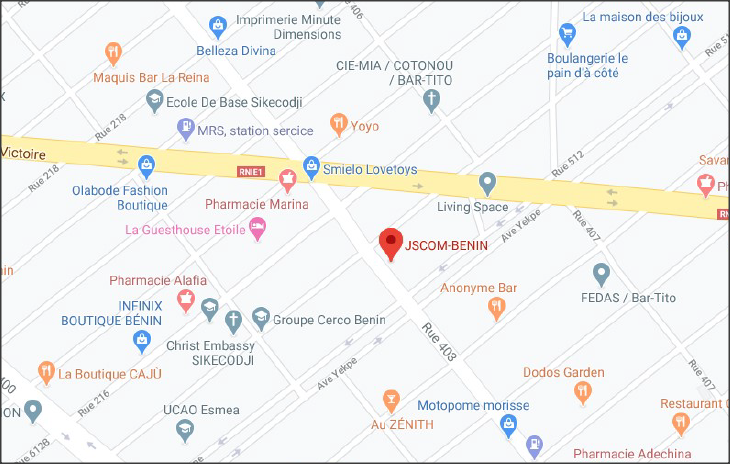
\includegraphics[scale=0.8]{figure/jscom-map.png}		
	\caption{Situation géographique de JScom, source Google Maps}		
	\label{Situation géographique de JScom}
	\end{figure}
		
	\subsection{Organisation}
	La société JSCOM dispose d'un peronnel très dynamique. Ce personnel sous la direction de son directeur lui a permis de gagner la confiance de ces clients. Cette confiance est fondée sur la qualité de ses prestations et le respect de ces engagements.
	
	\subsection{Domaine d'intervention}
	La société JSCOM intervient dans les domaines suivants :
	\begin{itemize}
		\item Développement de site web ;
		\item Développement d'application mobile et de bureau ;
		\item Mise en place des systèmes d'information structurée en entreprise ;
		\item L'implémentation des solutions électroniques de déclaration fiscale, du contrôle fiscal et de la facturation électronique normalisée et certifiée ;
		\item Formation en Windev

	\end{itemize}

	 %\subsection{Domaine d'intervention}
		%JScom intervient :
	%\begin{itemize}
		%\item Dans le développement des solutions sur mesure à l'intégration des systèmes d'informations
	%	\item Dans la formation en Windev et Webdev 
	%\end{itemize}
		
	%\section{Déroulement et observations}
\section{Démarche méthodologique}
	Au cours du stage, il a fallu :
	\begin{itemize}
		\item Faire une revue littéraire sur les notions du réseau informatique ;
		\item Prendre connaissance de la tâche à effectuer ;
		\item Nous référer aux connaissances reçues en classe ;
		\item Effectuer les opérations sur le terrain ;
		\item Faire le traitement au bureau ;
	\end{itemize}
			
\chapter{Cadre théorique et méthodologique}
	Dans ce chapitre, nous allons présenter le thème et toutes les notions fondamentales qui ont rapport au thème.
\begin{comment}
\section{Enoncé du problème}
	La communication est un outils indispensable pour l’apprentissage en milieux scolaires. Il faut une bonne communication pour faciliter les échanges et les activités  au sein de l’école. En temps qu’ élève à l’ENEAM, mes camarades et moi avons rencontrés quelques problèmes liés à la comminication. Nous avons été confrontés à des difficultés de communication  liées : 
\begin{itemize}
	\item à  la programmation des cours aux apprenants ;
	\item à l’effectivité ou non d’un cours ;
	\item aux échanges  entre étudiants sur les horaires des cours ;
	\item aux activités de groupe entre apprenants.
\end{itemize}

Ceci nous amène à rechercher les facteurs d’amélioration de la qualité de la communication à l’école. D’où la question fondamentale de recherche : \\
Quel facteur pourrait améliorer la communication à l’ENEAM ?
\end{comment}

\section{Enoncé du problème}
La communication est importante dans toute société car elle met en relation les hommes. Ainsi, la communication est au c\oe{}ur de toutes les activités menées à l’école. A l’école, la communication regroupe toutes informations utiles que l'administration peut mettre à disposition des étudiants, que les professeurs peuvent échanger avec leurs apprenants, de même que les apprenants peuvent s'échanger entre eux. Une bonne communication en milieu scolaire est donc essentielle à la réussite des apprenants. Cependant, durant nos années études à l'ENEAM, nous avons rencontré plusieurs obstacles dans la communication :
\begin{itemize}
	\item Le manque de communication entre étudiant des changements dans les horaires des cours ; 
	\item Le manque d’échanges entre étudiants sur les notions reçues ; 
	\item La mauvaise communication entre étudiants hors du cadre scolaire ;
	\item L’accès à certaines informations ; 
	\item La non-conformité ou la divergence des informations relayées par les étudiants ;
	\item La véracité de certaines informations en général diffusées par les étudiants.
	%\item Les difficultés de communication lors des activités de groupe entre étudiants.	
\end{itemize}
	En effet, l'administration dispose de courriels pour échanger en interne. En ce qui concerne les étudiants, les informations sont collées au tableau ou  relayées par les responsables de classe. De même, il est courant que les professeurs procèdent au réajustement de l'horaire des cours, or dans ces circonstances les étudiants ne sont pas tous informés des changements effectués. Il y'a dans ces conditions un déséquilibre dans la communication qui porte à réflexion.\\
Nous avons donc éprouvé le besoin de rechercher les facteurs d'amélioration de la qualité de la communication à l'école de façon spécifique à l'ENEAM. D'où la question fondamentale de recherche : \\
Quel facteur peut contribuer à améliorer la communication entre étudiants au sein de l'ENEAM?
	%Quel facteur pourrait contribuer à améliorer la communication  au sein de l'ENEAM?
\begin{comment} 
\section{Enoncé du probleme}
La bonne marche des actictés d’une école repose sur une bonne communication : communication verbale, non verbale, directe, indirecte. A l’ENEAM nous avons pu remarquer un réajustement de l’horaire des cours pour faire face à plusieurs contraintes : disponibilité des salles, des professeurs. Mais certains étudiants, par manque de communication ne sont pas informés des nouveaux horaires. Nous avons rencontrés des obstacles dans la communication qui sont liés :
\begin{itemize} 
	\item à la programmation des cours ;
	\item aux échanges entre étudiants ;
	\item aux activités de groupe entre étudiants.	
\end{itemize}
Ceci nous amène à rechercher les facteurs d’amélioration de la qualité de la communication à l’école. D’où la question fondamentale de recherche : \\
Quel facteur contribuerait à améliorer la communication au sein de l’ENEAM ?
\end{comment}
\begin{comment} 
	%J'ai enlevé beaucoup de problème % L'idée aussi est d'amener à combiner le numérique avec l'existent
	J'ai constaté qu'il a beaucoup d'incompréhensions dans la programmation des cours à ENEAM. Les étudiants s'embrouillent sur l'effectivité de la tenue des cours. De même quand on annule un cours les élèves sont parfois mal informés. %Souvent ils sont à l'école et attendent le professeur qui annonce qu'il ne viendra pas. 
	Souvent ils sont à l'école et s'amusent et perdent leur temps à ne rien faire. L'administration diffuse certaines informations qui sont sur support papier et sont collées. Et tout le monde n'est pas au courant; je me rappelle en 3\up{e} année, un de mes camarades est venu très en retard à une composition parce qu'il n'était pas informé de la date des évaluations. Que puis-je faire ? Les étudiants ont besoin d'un moyen de communication puissant pour discuter et ou s'échanger à propos des cours. Comme moyen, il a les réseaux sociaux. Les réseaux sociaux ne répondent pas à ce problème. En effet, on peut communiquer de façon illimitée par les réseaux sociaux, ce qui poussent les étudiants à dirent des inepties par ces canaux. Nous avons donc besoin d'un système qui va remplir plusieurs conditions :
\begin{itemize}
	\item Les professeurs pourront communiquer la programmation des cours aux apprenants de façon efficace ;
	\item Les élèves pourront échanger de façon simple ;
	\item Les administrateurs pourront surveiller le flux d'informations qui transite par le réseau ;
	\item L'administration pourra diffuser des informations et des communiqués ;
	\item L'administration pourra renforcer la qualité de service: on pourrait créer un canal spécial et périodique pour certaines procédures telles que les procédures de réclamation et autres services disponibles temporairement ;
	\item Un système de communication sûre, multi-utilisateurs, sécurisée. 
\end{itemize}

	\'Etudions les options dont on dispose. En informatique, on pourrait contribuer en réalisant une application, un réseau social.
Présentons ces avantages. Une bonne application peut répondre à tous les problèmes mentionnés ci-dessus mais la conception est une tâche bien pénible surtout lorsqu'on parle de sécurité, de système multi-utilisateurs, multitâches et d'administration. Il suffit pour s'en convaincre d'observer les médias sociaux qui existent : c'est beaucoup % j'ai enlevé d'ingénieurs et 
de technologies réunies. Nous voyons bien que cette solution bien que réalisable, pour qu'elle réponde à tous nos besoins, il faut beaucoup de ressources. Quand on dit ressources ici il y a les ressources matérielles, humaines, le temps, etc. Au vu de toutes ces disconvenues essayons de trouver une autre solution. Comme je suis un étudiant en administration réseaux, je vais essayer de parcourir parmi les solutions que proposent l'incroyable monde du réseau.

Prenons le mail. L'e-mail ou courrier électronique est un système de transmission de messages électroniques entre différents utilisateurs. Ce système achemine les messages entre deux nœuds reliés entre eux par le réseau internet. Par message électronique, on comprend des messages textes mais aussi des messages enrichis (c'est-à-dire des messages formatés dans un langage de description des données : HTML \label{ref:html} ), des fichiers joints ( documents, musique, vidéo) et tout autre type de fichiers. Le mail a plusieurs avantages :
\begin{itemize}
	\item C'est un réseau centralisé: les administrateurs peuvent donc surveiller le flux réseau, limiter le nombre de mails envoyés par les étudiants; ce qui empêche les apprenants d'envoyer des messages jugés inutiles ou des blagues sur le réseau. Plusieurs filtres peuvent être définis pour mieux analyser les données qui transitent sur le réseau ;
	\item Les membres de l'administration  peuvent envoyer le programme des cours, des devoirs aux étudiants, donc tout type d'information ;
	\item les élèves peuvent s'échanger entre eux sur les notions reçues ; 
	\item La sécurité est au point : le mail fait intervenir des protocoles réseaux standardisés et sécurisés qui répondent à tous les principes fondamentaux de la cryptographie. C'est un moyen de communication sûr lorsqu'il est bien configuré ;
	\item il a aussi des avantages personnels: l'apprentissage et l'exploration d'un riche et vaste domaine ainsi que la maîtrise de ces champs d'application.
\end{itemize}

	Au vu de ces avantages, je me propose de mettre en place un serveur de messagerie électronique.
Pour cela, je vais procéder étape par étape. Je vais donc mettre en place un serveur simple Linux, monter les disques durs, installer les services de bases DHCP, DNS, Apache,  MySQL, faire de la virtualisation, faire de la modélisation réseau grâce à GNS3, configurer le mail proprement avec les protocoles SMTP et IMAP, penser à la sécurité en définissant une politique de sécurité, en configurant les firewalls, en utilisant de la cryptographie (chiffrement symétrique, asymétrique, certificat, fonction de chiffrement de mot de passe),  mettre en place la supervision pour prévenir, détecter et corriger les problèmes, programmer également un petit site web d'administrations, écrire des scripts Bash. 
\end{comment} 

\section{Objectif}
	L'objectif est de mettre en place un serveur mail opérationnel pour l'ENEAM. De façon spécifique, il s'agit de déployer un serveur de messagerie et d'y proposer un accès par la technologie web.
	\section{Hypothèse}
	Les problèmes de communication liée à la programmation des cours sont dus à l'absence d'un moyen de communication innovant, combinant les technologies de l'information au sein de l'ENEAM.
	\section{Etude théorique}
		\subsection{Définition d'un serveur}
		Un serveur est un ordinateur qui fournit un ou plusieurs services aux clients. Les clients et le serveur communiquent grâce à des protocoles réseaux. En réseau, un protocole est un langage qui définit des règles, des conventions qui permettent aux ordinateurs (de façon générale, tout équipement électronique qui possède une carte réseau) de communiquer. Un serveur peut être également considéré comme un logiciel qui fournit un service à d'autres logiciels.

\subsubsection{Les caractéristiques d'un serveur}
Un serveur à généralement les caractéristiques suivantes :
\begin{itemize}
\item Un serveur est allumé 24h/24h ;
\item Très souvent, il ne dispose pas d'un écran, ni d'un clavier, ni d'équipements multimédias; % Un serveur peut avoir ;
\item Un serveur Linux n'a généralement pas d'interface graphique. Comme un serveur n'est pas souvent connecté à un écran, on préfère ne pas installer un environnement graphique ;
\item Un serveur utilise très souvent un système d'exploitation spécialisé.
\end{itemize}

\subsubsection{Quelques services}
Les serveurs assurent différents services parmi lesquels, nous pouvons citer :
\begin{itemize}
\item Transfert de fichier: NFS, Samba, FTP ;
\item Communication : Messagerie instantanée, téléphonie par IP ;
\item Authentification: annuaire LDAP ;
\item Web.
\end{itemize}

\subsubsection{Spécification d'un OS serveur}
	Un système d'exploitation de serveur (OS Operating System) est un système d'exploitation optimisé pour l'installation de logiciels serveurs. Les OS serveurs ont les caractéristiques suivantes:
\begin{itemize}
	\item Les OS serveurs ne sont pas configurés avec des fonctions de veilles. En effet les serveurs restent allumés tout le temps ;
	%\item Les OS serveurs n'ont pas d'interface graphique pour les systèmes Unix et Linux ;
	\item Les OS serveurs n'ont pas souvent d'interface graphique pour les systèmes Unix et Linux. En effet, ils peuvent avoir un environnement graphique mais on préfère ne pas l'installer puisqu'on y connecte pas de matériel graphique (écran) ;
	\item Ils peuvent gérer des ressources physiques énormes par rapport à un ordinateur personnel. Une machine serveur peut par exemple être dotée de plus 200 gigas (200 Go) de mémoires RAM. Il existe des services de support payants pour les entreprises.
\end{itemize} 
	
\subsection{Disque dur RAID et LVM}
RAID est un ensemble de techniques qui visent à répartir le stockage de données sur plusieurs disques physiques afin d'anticiper la défaillance des disques et de limiter les risques de pertes de données. Son principe est simple : on regroupe plusieurs disques pour constituer un seul disque dur visible par l'utilisateur. Ainsi lorsque l'un des disques se détériore, le disque endommagé peut être remplacé sans risque de perte de données. On distingue plusieurs architectures RAID :
\begin{itemize}
	\item Le RAID 0: dans cette architecture, si on prend deux disques, les deux travaillent en parallèle. Si un disque est détérioré toutes les données sont perdues ;
	\item Le RAID 1 : Pour deux disques durs physiques A et B, les données sont écrites simultanément sur les deux disques. Ainsi si A se gâte on peut continuer à travailler sans perte de données. Il suffit après de changer le disque A détérioré par un nouveau disque C pour ne pas risquer de perdre les données définitivement puisque le seul disque restant pourrait s'endommager ;
	\item Le raid 10: consiste à assembler au moins deux unités RAID 1 en un ensemble de RAID 0. Il faut donc un minimum de quatre disques et toujours en nombre pair. Il offre la sécurité puisque les données sont répliquées sur plusieurs grappes et améliorent la performance car les données sont écrites sur plusieurs disques.% Une grappe ainsi assemblée forme ainsi une unité logique qui sera associée avec d’autres grappes pour permettre un entrelacement comme c’est le cas d’un système RAID 0. La redondance des données dans chaque sous-unité permet de garantir leur sécurité, tandis que la répartition des données sur plusieurs unités logiques accélère la lecture et l’écriture.
	\item Le raid 5 : utilise au moins trois disques et répartit les données sur tous les disques en rajoutant des blocs de parité. Une donnée perdue peut être récupérée grâce aux blocs de parité. Si plus d'un disque s'endommage, on perd toutes les données. 
\end{itemize}

LVM (Logical Volume Management) permet la création et la gestion des volumes logiques sans perte de données. C'est un système qui permet par exemple de diminuer la taille d'un système de fichier pour pouvoir en agrandir un autre, sans se préoccuper de leur emplacement sur le disque. Les opérations de redimensionnement deviennent quasiment sans risque, contrairement au redimensionnement des partitions. Si un des volumes physiques est endommagé, alors l'ensemble des volumes logiques qui utilise ce volume physique est perdu. Pour éviter ce problème, il faut utiliser LVM sur des disques RAID par exemple.


\subsection{Serveur web APACHE}
Un serveur web est le service qui permet d'accéder à des pages web. Notre serveur de mail sera accessible par une interface web. Nous allons installer le serveur web Apache. Apache ou plus précisément HTTPD est le serveur web le plus populaire. Il est développé et maintenu par la fondation \emph{Apache}. Le serveur web Nginx sera utilisé comme reverse proxy\footnote{Un reverse proxy est un proxy qui filtre les requêtes de l'extérieur à destination d'un serveur interne. Il est utile pour la sécurité et les performances car il permet de gérer aussi un système de cache.}.

\subsection{Base de données}
Les données des utilisateurs doivent être stockées dans une base de données. Une base de données permet de stocker, de structurer, de gérer et d'accéder aux données de façon sûre, rapide et sécurisée. Un SGBD (Système de Gestion de Base de Données) est un logiciel qui manipule une base de données. Une base de données est un fichier ou un ensemble de fichier qui contient des données bien organisées qui peuvent être lues et manipulées par un SGBD à travers un langage informatique (langage de description ou langage de programmation). On distingue deux principaux types de bases de données.
 \begin{itemize}
 \item Les bases de données relationnels : les données sont stockées dans des tables et sont liées entre elle par des relations. Le langage SQL est utilisé pour interagir avec les données. Comme SGBD de ce type, on distingue MySQL, PostgreSQL, Oracle, et plein d'autres. En SQL, l'instruction: 
 \begin{minted}[frame = single, breaklines, autogobble, bgcolor=bg, label=SQL]{sql}
 SELECT `nom`, `prenom` FROM `utilisateur` WHERE `utilisateur`.`age` >=18 ; --Permet de sélectionner les nom, prénoms de tous les utilisateurs majeurs.
 \end{minted}
 \item Les bases de données NoSQL (Not Only SQL) : ceux sont des bases de données qui n'utilisent pas le modèle relationnel. Elles permettent la réplication des serveurs et de distribuer les données. On  peut citer à titre d'exemple Poids, MongoDB, Cassandra, ElasticSearch.
 \end{itemize}
 
\subsection{Modélisation avec GNS3}
La mise en place du projet nécessite de faire de la modélisation, c'est-à-dire représenter l'architecture réseau du projet de façon visuelle pour avoir un modèle, un plan représentatif de la solution à déployer. GNS3 est un logiciel libre qui permet de modéliser des architectures réseaux, de simuler des architectures réseaux, de visualiser et de tester le résultat grâce à la virtualisation.
%Pour mettre en place notre projet il va falloir le modéliser, c'est-à-dire représenter toute notre architecture réseau de façon visuelle pour avoir un modèle, un plan représentatif de la solution à déployer. GNS3 est un logiciel libre qui permet de modéliser des architectures réseaux, de simuler des architectures réseaux, de visualiser et de tester le résultat grâce à la virtualisation.
\subsection{Programmation}
%Un ordinateur ne comprend que le langage binaire, c'est-à-dire  1 et 0. Pour pouvoir donc donner une instruction à un ordinateur, il va falloir lui parler son langage qu'il comprend (le binaire). Comme le binaire n'est pas un langage accessible aux humains, on a créé les langages de programmation qui sont des instructions écrites dans un langage accessible à l'homme et qui seront ensuite soient lues, soient compilées, soient interprétées par des programmes spécifiques pour permettre à l'ordinateur de comprendre et donc de réaliser une tâche.
Les langages de programmation sont des instructions écrites dans un langage accessible à l'homme et qui sont ensuite soient lues, soient compilées, soient interprétées par des programmes spécifiques pour permettre à l'ordinateur de réaliser une tâche.
\subsubsection{HTML, CSS, PHP, JAVASCRIPT, JQUERY, BASH}
Les langages de programmation  web sont des langages de programmation qui interviennent dans le web. Il s'agit d'un ensemble de technologies qui permettent de créer des pages web dynamiques.
%C'est donc un ensemble de technologie qui permettent de créer des pages web dynamiques.
\paragraph{HTML} est un langage de description ou de balisage qui est dérivé du XML et qui permet d'écrire une page web statique. 
\paragraph{CSS} est un langage de description qui permet de rendre le contenu HTML attractif ( de faire la mise en forme du contenu).
\paragraph{PHP} est un langage orienté serveur, il va permettre de manipuler les données reçues par l'interface web d'administration du projet (site web).
\paragraph{JAVACRIPT ET JQUERY :} Le Javascript est le langage qui va nous permettre de rendre responsive le site web du coté client. Jquery est un framework du javascript, c'est un ensemble de lignes de code déjà implémenté qui va accélérer le développement de notre application.
\paragraph{BASH} est un langage de script qui permet d'exécuter des instructions sur un système d'exploitation Linux. Par exemple, un script bash peut être écrit pour éteindre un ordinateur à une heure donnée. Il est intégré dans tous les systèmes Linux et ne nécessite aucune installation. Il est essentiel car il va permettre de créer ou de supprimer les répertoires des utilisateurs, de vérifier l'état d'un service, d'arrêter ou de redémarrer un service.

\subsection{FTP} 
Le site d'administration développé va être envoyé sur le serveur grâce à un client graphique (comme FilleZila) qui utilise le protocole FTP. Le protocole FTP permet l'envoi et la réception de fichiers. Son usage est courant pour le téléchargement de fichiers et la majorité des dépôts Linux s'en sert pour le téléchargement des packages (apt le gestionnaire de paquets Debian télécharge les paquets sur des serveurs FTP).
%Pour envoyer le site d'administration que nous allons développer sur le serveur, nous allons utiliser un client graphique (comme FilleZilla nous n'allons pas utiliser le terminal mais plutôt utiliser le protocole d'envoi de fichier FTP et se servir d'un client FTP graphique (FilleZilla). Le protocole FTP permet l'envoi et la réception de fichiers. Il est très utilisé pour le téléchargement de fichiers. La majorité des dépots Linux utilisent le protocole FTP pour le téléchargement des packages (apt le gestionnaire de paquet Debian télécharge les paquets sur des serveurs FTP).
%J'ai oublié structure d'une adresse email
%\subsection{Structure d'une adresse email}
\subsection{Fonctionnement du mail}
La messagerie informatique fait intervenir plusieurs protocoles réseaux. Il a en effet le protocole SMTP qui permet d'envoyer le message et les protocoles IMAP et POP pour accéder aux données (les mails).
\subsubsection{SMTP}
Le serveur SMTP permet d'envoyer un mail. A titre d'exemple, si Toto (qui a pour adresse mail \textbf{toto@toto.com}s) veut envoyer un mail à Baké (qui a pour adresse \textbf{bake@gmail.com}), il va se produire les étapes suivantes :
\begin{itemize}
	\item Toto va se connecter depuis son poste (ordinateur, téléphone portable) à son serveur SMTP, rédiger le mail et l'envoyer ;
	\item Le serveur SMTP de Toto (Toto est l'émetteur ou expéditeur) avant  d'envoyer le mail, va vérifier  si le destinataire du mail (dans notre cas Baké) est sur le même serveur. En d'autres termes, il vérifie si l'expéditeur et le destinataire sont sur le même serveur. Il se sert de la partie nom de domaine de l'adresse email pour la vérification. Dans notre cas le serveur SMTP de Toto vérifie si Baké appartient à ce même serveur. La partie nom de domaine de toto est \textbf{toto.com} et de baké est \textbf{gmail.com} . Les deux ne sont pas identiques donc Toto et Baké sont sur deux serveurs SMTP différents ;
	\item Dans le cas où le destinataire appartient au serveur SMTP de l'émetteur, le serveur SMTP de l'émetteur va enregistrer directement le mail dans le dossier de réception des mails du destinataire qui est situé sur ce même serveur ;
	\item Dans le cas où l'expéditeur et le destinataire sont sur différents serveurs, le serveur SMTP de l'expéditeur va transmettre le mail à un autre serveur SMTP. Ce serveur va ensuite vérifier si le courriel lui est destiné. Si le courriel ne lui est pas destiné,  il va à son tour router le mail, c'est-à-dire envoyer le courriel à un autre serveur SMTP. Le mail sera routé jusqu'à arriver sur le serveur SMTP du destinataire. Le serveur du destinataire va stocker le mail dans le répertoire de réception du destinataire. Très souvent, il n'a pas de routage des mails et le serveur SMTP de l'expéditeur envoie directement le message au serveur SMTP du destinataire. Pour notre illustration, le serveur SMTP du domaine eneam.da va transmettre le mail au serveur SMTP du domaine gmail.com. Le serveur SMTP de gmail.com va réceptionner le mail dans le répertoire de Baké.
	%\item Dans le cas où l'expéditeur et le destinataire sont sur différents serveurs, le serveur SMTP de l'expéditeur va transmettre le mail au serveur SMTP du destinataire. Le serveur du destinataire va stocker le mail dans le répertoire du destinataire. Pour notre illustration, le serveur SMTP du domaine eneam.da va transmettre le mail au serveur SMTP du domaine gmail.com. Le serveur SMTP de gmail.com va réceptionner le mail dans le répertoire de Baké.
	%\item Le serveur SMTP de Baké va recevoir le mail de Toto et le stocker dans le répertoire personnel de Toto.	   
\end{itemize}
\begin{comment}
\begin{itemize}
	\item Toto va envoyer le mail depuis son poste à son serveur SMTP. 
	\item Le serveur SMTP de Toto va réceptionner le mail et vérifier s'il lui est destiné (il va vérifier si le destinataire du mail est sur ce serveur, c'est-à-dire si Baké appartient à ce serveur. toto@toto.com a pour domaine toto.com. et bake@gmail.com a pour domaine gmail.com. toto.com est différent de gmail.com donc les deux comptes mail ne sont pas sur le même serveur ). Si cette condition est vérifiée, il va enregistrer le mail dans le répertoire de réception des mails de Baké sinon il va relayer le mail vers le serveur SMTP de Baké. 
	\item Le serveur SMTP de Baké va recevoir le mail de Toto et le stocker dans le répertoire personnel de Toto.	   
\end{itemize}
\end{comment}
\begin{figure}[H]
\centering
\includegraphics[scale=1]{figure/"figure envoi SMTP.png"}
\caption{Principe du SMTP}
\label{Principer du SMTP}
\end{figure}

\subsubsection{IMAP}
La lecture des mails se fait par l'établissement d'une connexion au serveur. On utilise le protocole IMAP qui va se connecter au serveur, récupérer et afficher les mails dans un logiciel approprié (Mozilla Thunderbird, Yahoo mail, Zimbra, Rainloop).
	%Pour lire mes mails, je dois pouvoir accéder à mon serveur SMTP et lire les messages à distante. Pour cela on utilise le protocole IMAP qui va se connecter au serveur et récupérer les données et l'afficher dans le logiciel qui permet de lire les mails (un exemple Mozilla Thunderbird, Yahoo mail, Zimbra, Rainloop ). 
\begin{figure}[H]
\centering
\includegraphics[scale=1]{figure/"figure_reception_imap.png"} 
\caption{Réception d'un mail en IMAP}
\label{Reception d'un mail en IMAP}
\end{figure}
Lorsqu’un compte mail est configuré avec IMAP, le client email établit une connexion avec le serveur avant chaque consultation. On accède donc aux dossiers et mails dont le contenu sera chargé directement depuis le serveur sur demande. Avec ce protocole tous les messages peuvent être enregistrés sur le serveur et donc être accessibles jusqu’à leur suppression définitive. IMAP permet de ce fait la consultation des messages depuis n’importe quel ordinateur ou client connecté à internet. IMAP utilise le port TCP 143 et permet avec la TLS (Transport Layer Security) de fournir un accès sécurisé au serveur. Il est aussi possible d’avoir un accès sécurisé en SSL via le port 993.
\subsubsection{POP}
Avec le protocole POP (Post Office Protocol), le client de messagerie se connecte au serveur, copie tous les nouveaux messages présents sur sa boîte mail vers le disque dur de son ordinateur puis les courriels sont supprimés du serveur. Certains logiciels de courriel peuvent être configurés pour permettre de garder une copie des courriels sur le serveur. En cas d’interruption de la connexion, la gestion des mails se fait en hors-ligne. De plus, le protocole POP fournit un accès bloqué à la boîte mail c’est-à-dire qu’aucune autre connexion n’est permise en même temps que la connexion déjà en cours.% Les clients POP ont recours au port 110. Depuis la version 3 de POP il est possible de configurer un serveur POP qu’il fonctionne comme de l’IMAP.

\subsubsection{Différences entre IMAP et POP}
\cesure
\begin{table}[H]
	\centering
\begin{tabu}{|X[l]|X[l]|}
	\hline
	\centering \textbf{IMAP} & \centering \textbf{POP}  \\
	\hline
	Connexion au port 143 (993) & Connexion au port 110 (995) \\
	\hline	
	Connexion persistante (durable) & Connexion lors de l'extraction d'emails uniquement \\
	\hline
	Les emails sont conservés sur le serveur & Les emails sont supprimés immédiatement après avoir été téléchargés avec succès \\
	\hline
	Il est possible de charger les mails sur plusieurs clients & Un courriel ne peut être chargé que sur un seul client \\
	\hline
	Seuls les messages souhaités sont téléchargés & Tous les messages sont téléchargés \\
	\hline	
\end{tabu}
\end{table}
\nocesure

Il est conseillé de préférer le protocole IMAP au protocole POP car en plus de permettre l'accès multiple au serveur, le protocole IMAP rend possible le changement de client de messagerie sans risque de perte de données. De même IMAP synchronise automatiquement les messages et permet de gérer les dossiers du type \textbf{\og messages envoyés, spams, brouillons \fg{}}.

\begin{comment}
\subsubsection{IMAP}
	La lecture des mails se fait par l'établissement d'une connexion au serveur. On utilise le protocole IMAP qui va se connecter au serveur, récupérer et afficher les mails dans un logiciel approprié (Mozilla Thunderbird, Yahoo mail, Zimbra, Rainloop).
	%Pour lire mes mails, je dois pouvoir accéder à mon serveur SMTP et lire les messages à distante. Pour cela on utilise le protocole IMAP qui va se connecter au serveur et récupérer les données et l'afficher dans le logiciel qui permet de lire les mails (un exemple Mozilla Thunderbird, Yahoo mail, Zimbra, Rainloop ). 
\begin{figure}[H]
\centering
\includegraphics[scale=1]{figure/"figure_reception_imap.png"} 
\caption{Réception d'un mail en IMAP}
\label{Reception d'un mail en IMAP}
\end{figure}
Le protocole IMAP, contrairement à POP, ne se contente pas de relever les courriels, mais synchronise les messages, puisque les courriels restent sur le serveur. 
IMAP vous permet donc d’avoir accès à vos courriels depuis n’importe quel appareil (par exemple : plusieurs ordinateurs, tablette, téléphone intelligent).Par contre, l’espace de stockage disponible est celui défini par le serveur. Vous devrez de temps en temps trier et supprimer les messages qui ne vous sont plus utiles.
\end{comment}
\begin{comment}
	Le protocole POP permet aussi de récupérer vos courriels sur un serveur distant et de les télécharger sur votre ordinateur. 
Les courriels sont supprimés du serveur et sont téléchargés sur votre ordinateur. Certains logiciels de courriel vous permettent de garder une copie de vos courriels sur le serveur.
\end{comment}
\begin{comment}
Le protocole POP permet aussi de récupérer les mails. La différence fondamentale entre IMAP et POP est que IMAP est une connexion directe, unidirectionnelle  entre le serveur le client mail tandis que POP est une connexion bidirectionnelle.
\begin{itemize}
	\item Cela signifie qu'en IMAP les données sont sur le serveur et on y accède directement et toute modification faite sur les mails depuis le client mail impacte le serveur.%(est réalisée sur le serveur)
	En IMAP, la suppression des mails depuis un client mail est directement réalisée sur le serveur. De même, il est impossible d'avoir une copie locale des mails. On ne peut accéder aux mails déjà lu sans connexion internet. %En IMAP, si je supprime des mails depuis mon client mail, les mails sont aussitôt supprimés sur le serveur. De même avec IMAP, il est impossible d'avoir une copie local des mails . On ne peut donc accéder aux mails qu'on a déjà lu sans connexion internet.
	\item Avec POP, on réalise une copie locale de tous les mails qui sont sur le serveur. Ensuite, depuis le poste client, il est possible de modifier les mails sans enregistrer les changements sur le serveur. La lecture des mails déjà téléchargés est possible sans connexion internet.% On peut lire tous les mails téléchargés hors connexion.  
\end{itemize} 
Il est recommandé de préférer le protocole IMAP au protocole POP car la création de plusieurs copies locales d'un mail peut entrainer des confusions et conduire à effacer des données sur le serveur par inadvertance. A titre d'exemple Toto a récupéré en POP le mail identifié par \emph{MAIL1} avec son ordinateur portable. Il a commencé par répondre à ce mail et il a enregistré le brouillon de la réponse \emph{REPONSEMAIL1} en local sans l'envoyer sur le serveur. Il sort après sans son pc et réalise qu'il veut envoyer la réponse rédigée précédemment. Il se connecte au serveur mail avec son téléphone portable et ne retrouve par ce brouillon car le brouillon  \emph{REPONSEMAIL1} est enregistré sur son pc et non sur son serveur mail. Il est donc impossible d'envoyer cette réponse sans passer par son pc ; par contre en IMAP, Toto n'aurait pas rencontré ce problème puisque le brouillon \emph{REPONSEMAIL1} est enregistré sur le serveur. \\
\end{comment}
%	Il est recommandé de préférer le protocole IMAP au protocole POP car si on crée plusieurs copies locales d'un mail qui est sur le serveur, on peut facilement se tromper et écraser après des données sur le serveur sans le vouloir. Ou même supposons que j'ai récupéré en POP le mail identifié par \emph{MAIL1} avec mon ordinateur portable. J'ai naturellement commencé par répondre à ce mail et j'ai enregistré le brouillon de la réponse \emph{REPONSEMAIL1} sans avoir à envoyer la réponse au serveur. Je sors après sans mon pc et je réalise que je veux envoyer la réponse rédigée précédemment. Je me connecte à mon serveur mail avec mon portable et je ne retrouve par ce brouillon car le brouillon  \emph{REPONSEMAIL1} est enregistré sur mon pc et non sur mon serveur mail. Il m'est donc impossible d'envoyer cette réponse sans passer par mon pc ; ce qui n'allait  pas poser problème en IMAP puisque avec ce dernier le brouillon \emph{REPONSEMAIL1} aurait été enregistré sur le serveur. \\
	Le schéma complet de l'envoi et de la réception d'un mail avec le protocole IMAP.
\begin{figure}[H]
\centering
\includegraphics[width=483pt]{figure/"figure_envoi_reception_mail.png"} 
\caption{Résumé de l'envoi et de la réception d'un mail} \label{Résumé de l'envoi et de la reception d'un mai}
\end{figure}

\subsection{Sécurité}
La sécurité impose de ne pas faire confiance aux utilisateurs et aux données reçues des utilisateurs. Il convient d'établir des règles de sécurité strictes pour limiter les risques de mauvaises utilisations et de piratage informatique.
%En matière de sécurité on ne peut pas faire confiance aux utilisateurs et donc aux données reçues par les utilisateurs. Il faut alors établir des règles de sécurité strictes pour limiter les risques de mauvaises utilisations et de piratage informatique.
\subsubsection{Firewall}
Le firewall (pare-feu en français) est l'instrument qui va permettre de protéger le serveur contre l'extérieur. Il va installer une barrière entre notre serveur et l'extérieur. Par exemple, il sera possible au serveur d'aller sur internet (communication serveur vers extérieur) ou d'empêcher les utilisateurs depuis l'extérieur à communiquer avec le serveur\footnote{Il a un troisième cas : traverser le serveur. Dans ce cas le serveur joue le rôle d'un routeur.} (communication extérieur vers serveur). On distingue deux types de firewalls : les firewalls matériels et les firewalls logiciels (ou proxy).
\begin{itemize}
\item Le firewall matériel est une protection pour la couche 3 et 4 du modèle OSI. Il filtre le trafic réseau en lisant les entêtes IP et TCP ;
\item Le proxy est un firewall de niveau 6. Il filtre la couche applicative (couche application). Par exemple, il peut empêcher les étudiants à se connecter aux serveurs à certaines heures). Il peut servir aussi de cache.
\end{itemize}

\subsection*{Conclusion}
Nous allons installer un serveur Linux Ubuntu qui va contenir un certain nombre de services :
\begin{itemize}
	\item Un serveur SMTP et IMAP pour l'envoi et la réception des mails ;
	\item Un serveur web pour envoyer les mails depuis une application web (un webmail) ;
	\item Un site web d'administration pour créer des comptes mails et réaliser quelques tâches d'administration ;
	\item Une base de données pour sauvegarder les informations d'authentification ; 
	\item Un serveur FTP pour envoyer les données du site d'administration sur le serveur ;
	\item Un site web d'administration développé en PHP et en javascript ; 
	\item Des règles firewalls pour protéger le serveur ; 
	\item Un anti spam pour empêcher les spammeurs(Spamassassin) ;
	\item Une communication sécurisée par le chiffrement et les certificats ;
	\item Un serveur DNS qui gère le domaine eneam.da. Le webmail aura pour adresse \textbf{eneam.da} et le site d'administration \textbf{admin.eneam.da}.
\end{itemize}

\begin{comment}
	Nous allons :
\begin{itemize}
	\item Développer le site web d'administration  en PHP et en javascript. Les mails seront stockés sur un disque dur RAID\label{ref:raid}, LVM\label{ref:lvm} ;
	\item Ecrire des règles firewalls pour protéger le serveur ;
	\item Configurer un antispam pour empêcher les spammeurs (Spamassassin) ; % et limiter les risques de déni de service
	\item Sécuriser toute la communication par le chiffrage et des certificats ;
	\item Utiliser comme nom de domaine eneam.da\footnote{On pourra changer après ce nom en production.}. Le webmail aura pour adresse www.eneam.da et le site d'administration www.admin.eneam.da.
\end{itemize}
\end{comment}

%CHAPITRE CONCERNANT L'IMPLEMENTATION
\chapter{Implémentation du projet}
Ce chapitre est subdivisé en deux parties. La première partie va mettre en évidence la configuration des différents services et leurs fichiers de configuration. En seconde partie, la section \ref{ref:casConret} à la page \pageref{ref:casConret} va traiter d'un cas pratique de création et d'envoi de mails. 
%Je vais dans un premier temps me mettre dans la peau d'un administrateur système et configurer tous les services réseaux. Dans un second temps, dans la section \ref{ref:casConret} à la page \pageref{ref:casConret}, je vais me mettre à la place de l'utilisateur du système et je vais créer des comptes mails et envoyer des mails de façon simple et pratique. 
\section{Installation du serveur}
Nous utilisons comme OS \href{https://ubuntu-fr.org/telechargement?variante=server}{Ubuntu Server} et VMware comme hyperviseur\footnote{Un hyperviseur est un logiciel qui fournit un environnement virtuel pour installer un OS sans avoir un matériel réel. C'est grâce au hyperviseur que nous pouvons installer Linux et tester le projet depuis un poste Windows.}. Ubuntu est une distribution Linux gratuite et très populaire. Nous allons utiliser la version  LTS d'Ubuntu Server qui est disponible sur le site d'Ubuntu. La version LTS signifie Long Term Support et correspond à une version d'Ubuntu qui sort tous les 2 ans et qui bénéficie d'un support étendu sur 5 ans. Son intérêt est que cette version est stable et ne nécessite pas de mise à jour régulière. Le choix de l'hyperviseur VMware est lié au fait qu'il supporte une meilleure intégration avec l'émulateur d'architectures réseaux GNS3.%\footnote{Sera détaillé dans la suite}. 
 % L'avantage repose sur le fait que c'est une version stable qui ne nécessite pas de mise à jour régulière. Le choix de l'hyperviseur VMware est lié au fait qu'il supporte une meilleure intégration avec l'émulateur d'architectures réseaux GNS3.%\footnote{sera détaillé dans la suite}. 
%L'avantage est qu'on ne va pas s'embêter avec des mises régulières comme avec un OS standard. Le choix de l'hyperviseur VMware est axé sur le fait qu'il supporte une meilleure intégration avec l'émulateur d'architectures réseaux GNS3.%\footnote{Sera détaillé dans la suite}. 
%\subsection{Installation du serveur}

Nous suivons à ce niveau les instructions de Lavanant dans son cours \textbf{montez un serveur de fichiers sous linux}.
La première étape est l'installation de l'hyperviseur VMware workstation. Pour cela,  il faut :
\begin{itemize}
	\item Se rendre sur le site de VMware en  utilisant le lien \url{https://www.vmware.com} ; % cliquant \href{https://my.vmware.com/en/web/vmware/free}{ici} ;
	\item Télécharger, installer et ouvrir le logiciel. La version en anglais est utilisée ; 
	\item Ouvrir l'onglet File ensuite "New virtual Machine". Une fenêtre s'ouvre et il faut suivre le guide durant la configuration de la nouvelle machine virtuelle. Les différentes étapes d'ajout d'une machine virtuelle sont disponibles sur le site de VMware. La machine virtuelle serveur a les configurations suivantes : 1 Go de mémoire RAM, 40Go de stockage de masse (disque dur).
\end{itemize}
	%On installe d'abord l'hyperviseur VMware workstation. Pour cela rien de plus simple on se rend sur le site de VMware en cliquant \href{https://my.vmware.com/en/web/vmware/free}{ici}. On télécharge et installe le logiciel. On ouvre le logiciel. J'utilise la version en anglais de VMware. On ouvre l'onglet File ensuite "New virtual Machine". Une fenêtre s'ouvre et nous suivons le guide durant la configuration de la nouvelle machine virtuelle. Les étapes d'ajout d'une machine virtuelle sont disponibles sur le site de VMware. Nous avons normé la machine virtuelle serveur et elle à les configurations suivantes 1 Go de mémoire RAM, 40Go de stockage de masse (disque dur).

Il faut ensuite :
\begin{itemize}
	\item Démarrer la machine virtuelle \textbf{serveur} avec le disque Ubuntu Server qui est téléchargé en utilisant le lien \url{https://ubuntu-fr.org/telechargement} pour commencer l'installation ; 
	\item Suivre les instructions (choisir la langue, le clavier, configurer le réseau en DHCP). A la fin de l'installation le système demande de redémarrer ;
	\item  Après redémarrage, entrer le nom d'utilisateur et le mot de passe. Il faut configurer le réseau. 
\end{itemize}
	%On démarre la machine virtuelle \emph{\textbf{"serveur"}} avec le disque virtuel Ubuntu Server qu'on a téléchargé \href{https://my.vmware.com/en/web/vmware/free}{ici} pour démarrer l'installation. On suit les instructions (on choisit la langue, le clavier, on configure le réseau en DHCP). A la fin de l'installation le système nous dit de redémarrer. Après redémarrage, on entre le nom d'utilisateur et le mot de passe. Il faut configurer le réseau. 

La configuration du réseau nécessite d'avoir d'interfaces réseaux dans la machine virtuelle. Voici les étapes : 
\begin{itemize}
	\item Eteindre la machine virtuelle avec la commande 
	\begin{exempleConsole}
		sudo shutdown now 
	\end{exempleConsole}
	\item Dans VMWare, éditer les paramètres de la machine virtuelle et lui ajouter un adaptateur réseau configuré sur NAT. La NAT va permettre à la machine d'avoir accès à internet\footnote{L'accès à internet sera modifié après lors de la configuration avec GNS3.} ;
	\item Démarrer la machine et taper la commande
	\begin{exempleConsole}
	netplan apply
	\end{exempleConsole}
\end{itemize}
	
%Dans VMWare on édite les paramètres de la machine virtuelle et on lui ajoute % deux adaptateurs réseaux en veillant à bien cocher la case Custom et choisir VMnet2 pour le premier adaptateur et pour le second on choisit NAT.
%un adaptateur réseau (on choisit NAT). La NAT va permettre à notre machine d'avoir accès à internet\footnote{ l'accès à internet sera modifié pour au moment des configurations avec GNS3}. On démarre la machine. On tape la commande
%\begin{exempleConsole}
%netplan apply
%\end{exempleConsole}

\section{Gestion du stockage de fichier}
	Un disque dur spécial est utilisé pour stocker toutes les données liées aux mails que le serveur va contenir.
	% Nous allons configurer un disque dur spécial pour les données liées aux mails que le serveur va contenir.
\subsection{Système de fichier}
Un fichier est un contenu (ou un conteneur de données) binaire qui porte un nom et a souvent une extension qui permet de le distinguer. Ainsi, il est facile de reconnaître une image par son extension jpeg ou un document word par docx. Les fichiers sont stockés sur un support de masse (disque dur, carte mémoire). Un système de fichier est un index qui définit comment les fichiers sont stockés et organisés sur un disque afin de permettre et de faciliter l'accès aux différents fichiers. On distingue différents systèmes de fichiers FAT32, NTFS, EXT3, EXT4. EXT4 est l'actuel système de fichier qui est utilisé sur Linux. Il n'est pas compatible Windows (Windows ne supporte pas nativement le système de fichier EXT4). Donc pour stocker des informations sur un disque dur, il faut d'abord le préparer par la création du système de fichier et le formatage du disque. % Cela se fait par la création du système de fichier et le formatage du disque dur.
%	Toutes les données contenues dans un ordinateur sont du binaires( suite de 0 et 1). Il n'a aucun moyen pour un homme de distinguer alors les données. Pour cela on a créé les fichiers. Un fichier est alors un contenu (ou un conteneur de données) binaire qui porte un nom et a une extension qui permet de le distinguer. Ainsi, il est facile pour un homme de reconnaître une image par son extension jpeg ou un document word par docx. Les fichiers sont stockés sur un stockage de masse (disque dur, carte mémoire). Un système de fichier est un index qui définit comment les fichiers sont stockés et organisés sur le stockage afin de permettre et faciliter l'accès aux différents fichiers. On distingue différents systèmes de fichiers fat32, NTFS, ext3, ext4. EXT4 est l'actuel système de fichier qui est utilisé sur Linux. Il n'est pas compatible Windows, c'est-à-dire que Windows ne supporte pas le système de fichier EXT4. Donc pour pouvoir stockés des informations sur un disque dur, il faut d'abord le préparer. Cela se fait en créant le système de fichier puis en formatant le disque dur.
\subsection{Ajout de disque dur au serveur}	
\begin{itemize}
	\item Eteindre le serveur s'il est allumé. Dans les paramètres de la machine virtuelle, nous ajoutons trois disques de 2 giga ;
	\item Redémarrer la machine et exécuter la commande :
	\begin{exempleConsole}
		ls -la /dev/sd* 
	\end{exempleConsole}
	\item Vérifier la taille de chaque disque avec la commande
	\begin{exempleConsole}
	gdisk dev/sdb
	\end{exempleConsole}
	Dans gdisk, afficher la structure du disque pour vérifier que le stockage du disque est effectivement de deux giga. Taper q  pour quitter. Répéter la commande pour  les deux autres disques durs montés ;
 	\item Créer le RAID 1 avec la commande  
	\begin{exempleConsole}
	mdadm --create /dev/md0 --level=raid1 --raid-devices=2 /dev/sdb /dev/sdc spare-devices=1 /dev/sdd
	\end{exempleConsole}
	\item Afficher les détails sur le nouveau disque RAID créé et copier l'identifiant UUID
	\begin{exempleConsole}
		mdadm --query --detail /dev/md0
		/dev/md0:
				   Version : 1.2
			 Creation Time : Wed Dec 25 14:33:47 2019
				Raid Level : raid1
				Array Size : 2094080 (2045.00 MiB 2144.34 MB)
			 Used Dev Size : 2094080 (2045.00 MiB 2144.34 MB)
			  Raid Devices : 2
			 Total Devices : 3
			   Persistence : Superblock is persistent
		
			   Update Time : Tue Mar 10 11:18:38 2020
					 State : clean
			Active Devices : 2
		   Working Devices : 3
			Failed Devices : 0
			 Spare Devices : 1
		
		Consistency Policy : resync
		
					  Name : serveur:0  (local to host serveur)
					  UUID : 1bf998cb:0b420815:25812e34:403d63c5
					Events : 26
		
			Number   Major   Minor   RaidDevice State
			   0       8       16        0      active sync   /dev/sdb
			   1       8       32        1      active sync   /dev/sdc
		
			   2       8       48        -      spare   /dev/sdd
		
	\end{exempleConsole}
	\item  Ajouter la ligne suivante dans le fichier /etc/mdadm/mdadm.conf pour que le disque dur ne change pas de nom lors du prochain démarrage du système 
	\begin{exempleConsole}
	ARRAY /dev/md0 level=raid1 num-devices=2 spares=1 UUID=1bf998cb:0b420815:25812e34:403d63c5 devices=/dev/sdb,/dev/sdc,/dev/sdd
	\end{exempleConsole}
	\item Pour que les modifications soient effectives au prochain démarrage du système, faire
	\begin{exempleConsole}
	sudo update-initramfs -u
	\end{exempleConsole}
	\item Passer au partitionnement du nouveau disque avec LVM
	\begin{exempleConsole}
	sudo pvcreate /dev/md0
	sudo vgcreate raid-volume /dev/md0 
	sudo lvcreate --name data --size 2000M raid-volume
	\end{exempleConsole}
	\item Créer le dossier de montage puis monter la partition \emph{\textbf{data}} dans ce dossier 
	\begin{exempleConsole}
	mkdir -p /externe
	mount -t ext4 /dev/raid-volume/data /externe
	\end{exempleConsole}
	\item Rendre automatique le montage de la partition à chaque démarrage du système. Pour cela, éditer le fichier /etc/fstab et ajouter la ligne
	\begin{exempleConsole}
	/dev/raid-volume/data /externe ext4 defaults 0 0
	s\end{exempleConsole}
\end{itemize} 
	%On éteint le serveur. Puis on va dans les paramètres de la machine virtuelle ensuite on ajoute trois disques de 2 giga configurés en SCSI\footnote{Est une spécification matérielle des disques}.\\
%On redémarre la machine ensuite on exécute les instructions suivantes : \\
%On affiche la liste des disques durs. 
\section{Configurer le LAMP}

Dans cette section, Nous allons installer PHP, MariaDB qui est un fork\footnote{C'est quand des développeurs d'un logiciel en général libre n'étant plus d'accord pour continuer le projet se séparent et créent leur propre version du logiciel à partir du code source de départ.} de MySQL. Le cours  \textbf{gérez votre serveur linux et ses services de Lavanant
} dont nous allons nous inspiré traite correctement de la configuration du LAMP.
%On va installer PHP, MariaDB qui est un fork\footnote{C'est quand des développeurs d'un logiciel en général libre n'étant plus d'accord pour continuer le projet se séparent et créent leur propre version du logiciel à partir du code source de départ.} de MySQL.
\begin{exempleConsole}
sudo su
apt-get update #Pour mettre à jour le cache local
apt-get install apache2 libapache2-mod-php php-fpm mysql-server libapache2-mod-rpaf
#Pour activer les modules apache nécessaires
sudo a2enmod proxy_fcgi setenvif
sudo a2enconf php7.2-fpm
sudo a2dismod php7.2 mpm_prefork
sudo a2enmod mpm_event
sudo systemctl restart apache2
\end{exempleConsole}

\subsection{Gestion de Apache}
Nous changeons les ports sur lesquels écoute Apache httpd et il écoutera en local (l'interface localhost) sur 7080 pour le HTTP et 7443 pour le HTTPS. L'avantage est que notre serveur apache n'est pas exposé à l'extérieur. On verra seulement notre reverse-proxy Nginx de l'extérieur. Nous modifions le fichier /etc/apache2/ports.conf
\exempleConsoleFileBash{source/apache-ports.conf}
Nous allons configurer les virtualhosts (c'est-à-dire les deux sites web qui seront hébergés sur le serveur). Ces sites seront sécurisés avec des certificats auto-signés\footnote{Un certificat auto-signé est un certificat qui n'est pas créé par une autorité de certification.}.\label{ref:rainloop}
Nous créons le fichier /etc/apache2/site-available/www.eneam.da.conf ; il est associé au client webmail qui va lire les courriers.
\cesure
\exempleConsoleFile{source/www.eneam.da.conf}
\nocesure
Nous créons le fichier /etc/apache2/site-available/www.admin.eneam.da.conf ; il est associé au site d'administration. 
\cesure
\exempleConsoleFile{source/www.admin.eneam.da.conf}
\nocesure
Nous créons aussi les répertoires /externe/www/html/www.admin.eneam.da/logs/ récursivement.
\begin{exempleConsole}
mkdir -p /externe/www/html/www.admin.eneam.da/logs/ /externe/www/html/www.admin.eneam.da/public_html/
\end{exempleConsole}
Nous n'activons pas ces virtualhosts pour éviter une erreur d'Apache puisque leurs répertoires respectifs n'ont pas été créés.
%Nous n'avons pas activé ces virtualhosts pour le moment sinon Apache va sortir une erreur.
\subsection{Gestion de Nginx}
\begin{exempleConsole}
sudo apt-get install nginx libapache2-mod-rpaf
\end{exempleConsole}

Il faut créer les  \textbf{server blocs}\footnote{Dans Nginx, les virtualhosts sont appelés des servers blocs.} associés à nos virtualhosts. Pour le premier /etc/nginx/site-available/www.admin.eneam.da :
\exempleConsoleFileBash{source/www.admin.eneam.da}
Le fichier /etc/nginx/site-available/www.eneam.da :
\exempleConsoleFileBash{source/www.eneam.da}

\subsection*{Résumé}
En somme, nous avons configuré un serveur web Nginx accessible depuis l'extérieur. Lorsqu'on va se connecter aux différents sites depuis un navigateur, les requêtes (HTTP et HTTPS pour être précis) sont envoyées à Nginx. Nginx filtre  ces requêtes et va ensuite rediriger les requêtes en interne vers Apache. Apache en traitant ses requêtes, va déléguer la gestion des scripts PHP au processus FastCGI \emph{\textbf{PHP-FPM}}. Tout ceci se fait de façon transparente pour l'utilisateur.
\begin{figure}[H]
	\centering
	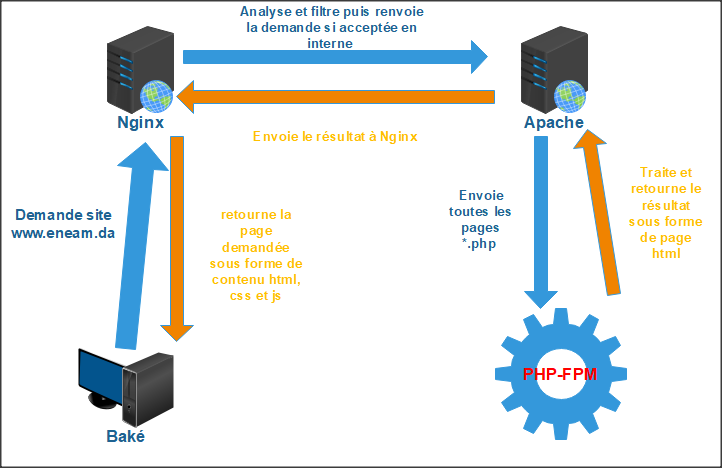
\includegraphics[scale=0.7]{figure/resume-fonctionnement-web-eneam.png}
	\caption{Résumé du fonctionnement web du réseau \textbf{projetmail}}
\end{figure}
\section{Modélisation de l'architecture réseau avec GNS3}
Pour cette étape, nous suivons les instructions de Motta dans son cours simulez des architectures réseaux avec gns3.
Il faut: 
\begin{itemize}
	\item Télécharger les logiciels GNS3  et GNS3 VM sur le site officiel de GNS3 et installer GNS3 ;
	\item Lancer le logiciel VMWare et cliquer sur Fichier puis sur  ouvrir fichier ;
	\item Choisir le fichier GNS VM au format ova téléchargé. Une nouvelle machine virtuelle va être ainsi installée. Il faut ensuite importer cette machine dans le logiciel GNS3 ;
	\item Lancer  GNS3. Menu Edit -> Préférences -> GNS3 VM ;
	\item Cocher la case  “Enable the GNS3 VM” et sélectionner “VMware Worstation/Player” dans le champ Virtualize engine ;
	\item Cliquer sur Refresh et GNS3 VM apparaît dans VM name ;
	\item Cliquer sur Apply ;
	\item Ajouter notre machine Linux \textbf{serveur} de VMware pour l'utiliser lors de la modélisation. Pour cela, se rendre dans Preferences -> VMware -> VMware VMs -> new. Une fenêtre apparaît. Cocher run this VMware VM on my local computer puis next ;
	\item Dans VM list, choisir la machine serveur, un clic sur le bouton finish.
\end{itemize}

\subsection{Description du schéma}
\begin{figure}[H]
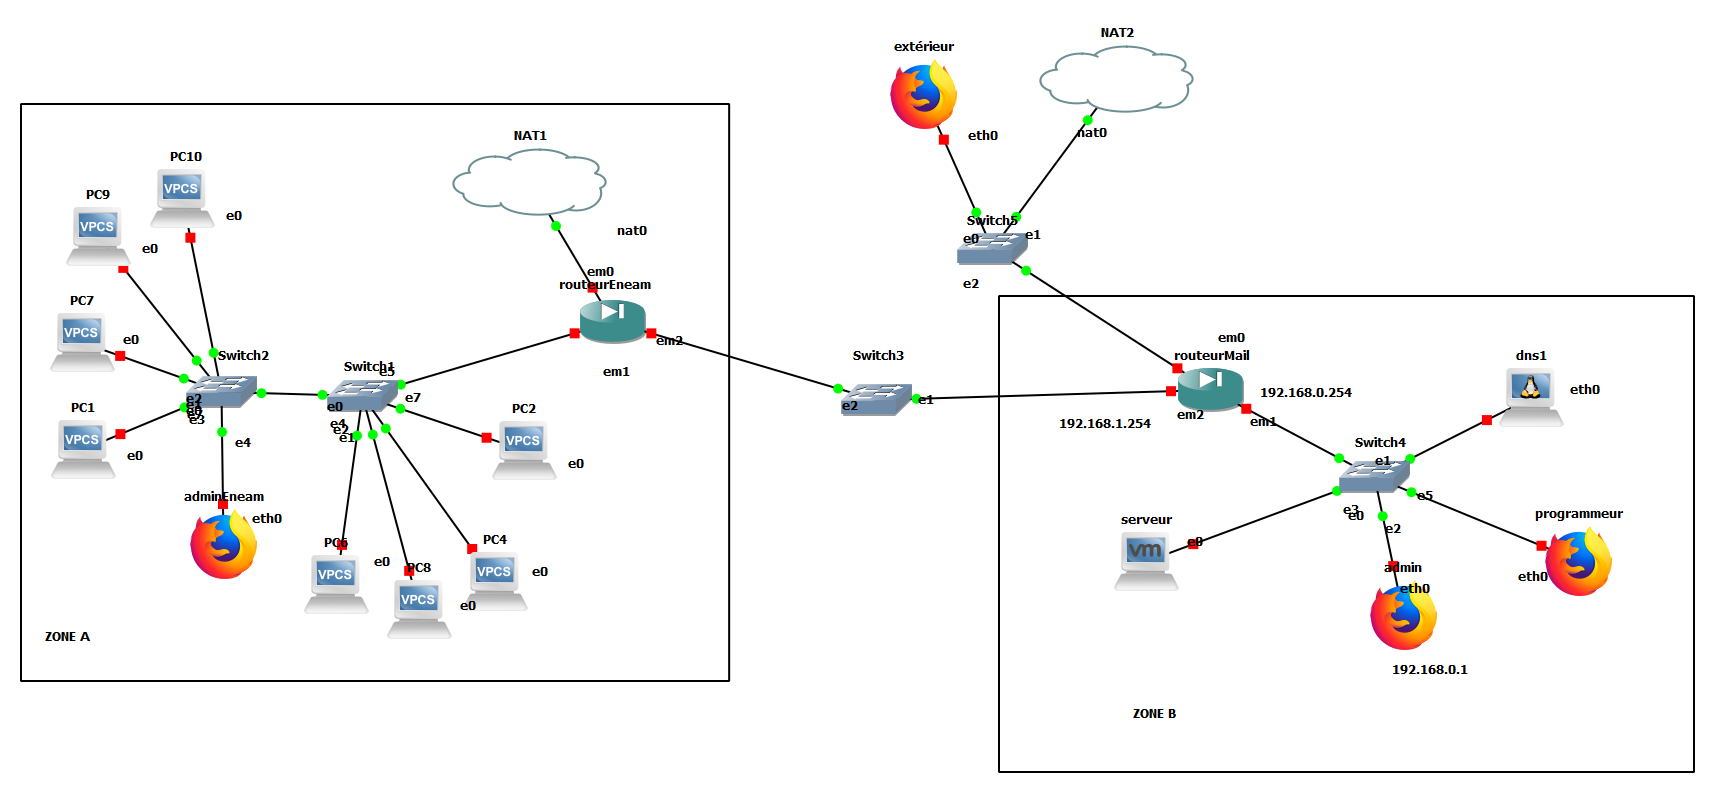
\includegraphics[width=520pt]{figure/topologie_gns3.png}
\centering
\caption{Topologie de notre projet dans GNS3}	
\end{figure}
Le réseau est séparé en deux grandes parties: la zone A et la zone B
%Nous avons opté pour un modèle générique. Le réseau est séparé en deux grandes parties: la zone A et la zone B
\begin{itemize}
\item La zone A : représente le réseau existant de l'ENEAM. Il est géré par \emph{\textbf{routeurEneam}} et est relié au routeur routeurMail. La configuration de cette zone ne nous intéresse pas. Elle permet de mieux comprendre l'architecture du projet. En effet, le projet est générique car il peut s'adapter à tout type d'organisation existante sans toucher au système d'information\footnote{Un système d'information est un ensemble de ressources matérielles, humaines qui permet de collecter, de stocker, de traiter et de diffuser l'information.} existant ;% Elle permet de mieux comprendre l'architecture du projet et de comprendre que le projet est générique car il peut s'adapter à tout type d'organisation existante sans toucher au système d'information\footnote{Un système d'information est un ensemble de ressources matérielles, humaines qui permet de collecter, de stocker, de traiter et de diffuser l'information.} existant ;
\item La zone B: le nouveau réseau relié par le routeur routeurMail ;
L'avantage d'une telle architecture est que l'administrateur du réseau de l'ENEAM peut communiquer avec le réseau mail à travers un tunnel (VPN) s'il est configuré ;
\item \textbf{routeurEneam} procède trois interfaces réseaux : em1 dans son réseau local, em2 qui le relie à routeurMail et em0 pour le WAN ;
\item \textbf{routeurMail} de même à trois interfaces ;
\item \textbf{dns1} est un docker\footnote{Est un conteneur qui contient un service et toutes les dépendances de ce dernier. Il permet d'isoler le service qu'on veut déployer (ici DNS) sans avoir à s'encombrer d'autres services dont on n'a pas besoin. Sans un docker, on aurait à installer un autre serveur Linux juste pour le DNS mais qui contient déjà plein de programmes dont nous n'avons  pas besoin. En somme un docker contient le strict minimum.} qui contient un petit serveur DNS qui va servir à la résolution dynamique des noms de domaine au sein du réseau local ;
\item \textbf{serveur :} c'est notre serveur Ubuntu installé depuis VMware ;
\item \textbf{routeurMail} et \textbf{routeurEneam} sont des routeurs Pfsense\footnote{Est un routeur firewall open source.} ;
\item \textbf{NAT2} permet de connecter routeurMail à internet et de pouvoir simuler l'accès de notre architecture à internet. Notre routeur aura un adressage privé (pour em0) ce qui n'est pas le cas dans la réalité puisque em0 devait avoir une adresse publique directement accessible sur internet. En effet, la modélisation avec GNS3 nous impose de faire comme cela ;
\end{itemize}

Les étapes de la création du projet :
\begin{itemize}
\item Créer un nouveau projet "projetmail" ;
\item Ajouter tous les équipements à notre topologie ;
\item \item Renommer tous les équipements ajoutés ;
\item Démarrer et configurer routeurEneam ;
\item Configurer le serveur DNS sur le poste \textbf{dns1} ;
\item Accéder à routeurEneam depuis le poste admin et configurer la NAT et le port forwading (redirection de port en français). Pour cela:
	\begin{itemize}
		\item Depuis le poste \textbf{admin}, ouvrir le navigateur Firefox ;
		\item Entrer l'adresse 192.168.0.254 et accéder à routeurEneam. Les identifiants par défaut sont admin et le mot de passe pfsense. Changer le mot de passe par défaut.
		\begin{figure}[H]
		\centering
		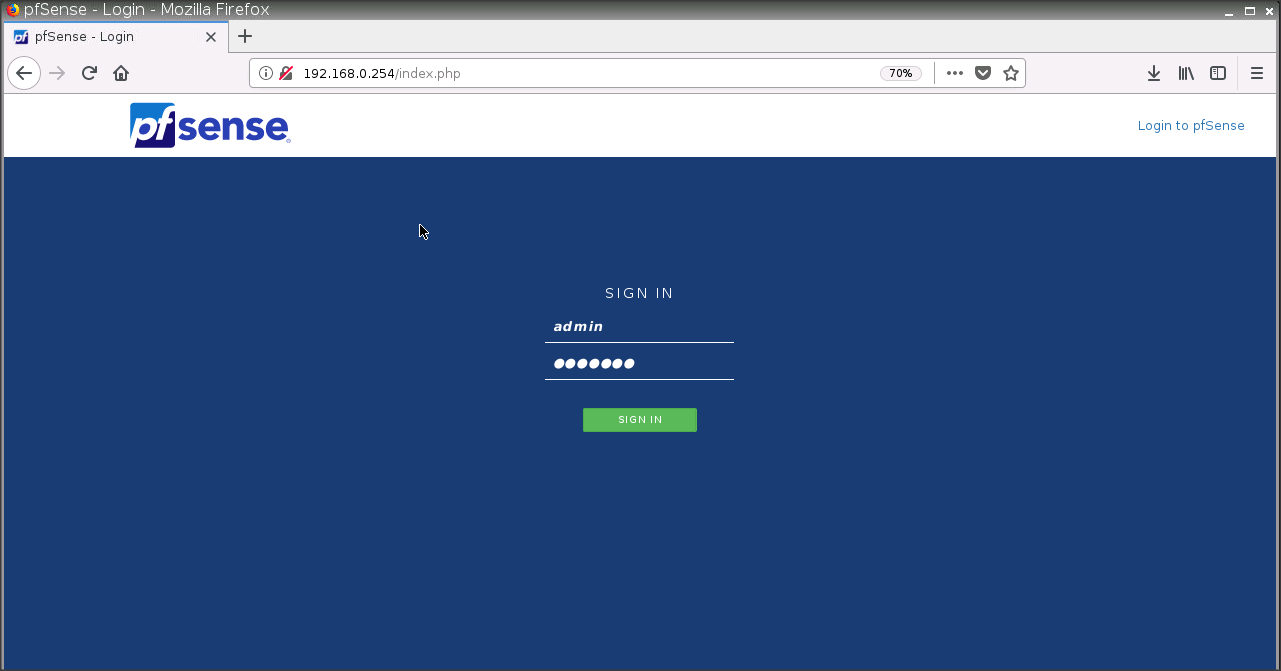
\includegraphics[width=483pt]{figure/pfsense_login.png}
		\caption{Connexion à pfsense par un navigateur}	
		\end{figure}	 	
	\end{itemize}
	Cette configuration va permettre d'accéder au mail par le webmail mais aussi d'y accéder par d'autres clients mails tels que Mozilla Thunderbird puisque que les ports STMP et IMAP sont ouverts vers l'extérieur. L'intérêt est qu'il serait possible de s'envoyer des mails sans passer par un client webmail installé sur le serveur.
%Ce qu'on a fait va permettre d'accéder au mail par le webmail mais aussi d'accéder par d'autres clients mail tels que Mozilla Thunderbird puisqu'on a rendu directement les ports STMP et IMAP ouverts vers l'extérieur. Si on fermait ces ports, il serait impossible de s'envoyer des mails sans passer par un client webmail installé sur le serveur
\begin{figure}[H]
\centering
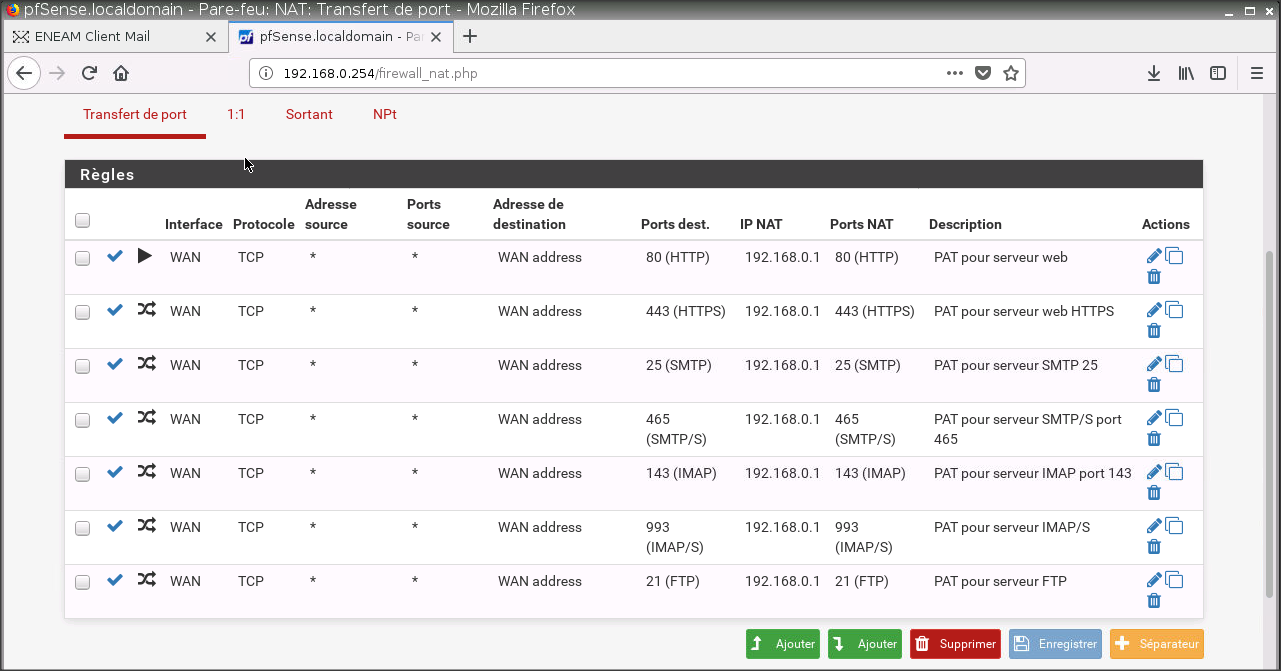
\includegraphics[width=483pt]{figure/figure_routeurMail_configuration_pat.png}
\caption{Configuration du port forwarding}
\label{Configuration du PAT}
\end{figure}
\item Il faut modifier les interfaces réseaux de notre serveur nommé \emph{\textbf{serveur}}. Pour cela dans VMware, on le configure pour qu'il ait deux interfaces réseaux ; l'une représente son interface dans lequel il est connecté dans GNS3 (e0 selon notre schéma) et la seconde interface est configuré en Host-Only\footnote{En effet, le site d'administration est codé sur notre machine physique Windows, il faut un moyen pour pouvoir envoyer le site sur le serveur virtuel, alors nous avons configuré un réseau privé entre le serveur de VMware et notre ordinateur Windows.}. Nous créons aussi le fichier /etc/netplan/60-lan\_statique.yaml pour configurer les interfaces du serveur.
%\exempleConsoleFileYAML{source/60-lan-statique.yaml}
\begin{exempleConsole}
network:
    renderer: networkd
    ethernets:
        ens33:
            dhcp4: no
            dhcp6: no
            gateway4: 192.168.0.254
            addresses: [192.168.0.1/24]
            nameservers:
                    search: [eneam.da]
                    addresses: [192.168.0.5,8.8.8.8]
        ens34:
            dhcp4: true      
    version: 2

\end{exempleConsole}

\end{itemize}

% peut servir à supprimer plus tard
%Postfix est un serveur SMTP. C'est donc lui qui va servir à l'envoi des mails
%Prenons le poste PC1 du réseau em1 s'il veut envoyer un mail à  jean@eneam.da
%depuis son poste il passe par internet. Il n'a pas communication directe entre les deux routeurs pour des  utilisateurs locaux.
%Il se connecte au serveur mail
\subsection{Configuration des équipements}

\section{Installation Postfix}
L'installation du serveur SMTP Postfix va se faire toujours avec notre gestionnaire de paquet apt
\begin{exempleConsole}
apt-get install postfix  postfix-mysql #et on reponds aux boîtes de dialogues qui s'affiche
\end{exempleConsole}

Les fichiers de configuration de postfix sont dans le dossier /etc/postfix/.
Nous réalisons une copie des fichiers de configuration avant toute modification.
Nous modifions le fichier /etc/postfix/main.cf
\fussy
\exempleConsoleFile{source/postfix-main.cf}
\nocesure
Dans ce fichier :
\begin{itemize}
	\item Le serveur postfix écoute sur IPV4 et IPV6 ;
	\item La partie SASL AUTHENTIFICATION renforce la sécurité du serveur. En effet, SASL est un protocole qui permet de sécuriser une connexion non sécurisée ;
	\item La partie TLS renforce la sécurité du serveur. SSL est un protocole qui va aussi permettre de sécuriser le serveur ;
	\item Toujours pour la sécurité nous utilisons des certificats auto-signés ; 
	\item La propriété virtual\_mailbox\_domains = mysql:/etc/postfix/sql/mysql-virtual-mailbox-domains.cf définit le fichier qui va contenir la directive de connexion à notre base de données MySQL plus précisément MariaDB ;
	%\item virtual\_mailbox\_maps = mysql:/etc/postfix/sql/mysql-virtual-mailbox-maps.cf.	
	\item La partie utilisation de boîte virtuelle va permettre d'utiliser les virtualhosts ; c'est-à-dire des comptes mails virtuels qui ne représentent pas les mails des utilisateurs réels de la machine \textbf{serveur}. L'utilisateur vhosts est créé par la commande
	\begin{exempleConsole}
	groupadd -g 5000 vhosts 
	useradd -g vhosts -u 5000 vhosts -d /externe/mail/vhosts -s /bin/false -m
	\end{exempleConsole}
\end{itemize}

Le fichier mysql-virtual-mailbox-domains.cf contient :
\begin{exempleConsole}
user = messagerieUser
password = amettre
hosts = 127.0.0.1
dbname = messagerie
query = SELECT 1 FROM virtual_domains WHERE name='%s'
\end{exempleConsole}

Le fichier mysql-mailbox-map contient :
\begin{exempleConsole}
user = messagerieUser
password = xxxxxxx
hosts = 127.0.0.1
dbname = messagerie
query = SELECT maildir FROM virtual_users WHERE email='%s'
\end{exempleConsole}

Le certificat est créé grâce à la bibliothèque cryptographique openssl :
\begin{exempleConsole}
openssl req -x509 -nodes -days 365 -newkey rsa:2048 -keyout /etc/ssl/private/dovecot-autosigne.key -out /etc/ssl/certs/dovecot-autosigne.crt
\end{exempleConsole}

Nous modifions le fichier master.cf. Il va permettre de renforcer la sécurité et d'obliger le serveur à accepter que des connexions sécurisées.
\cesure
\exempleConsoleFile{source/postfix-master.cf}

Les directives spamassassin permettent d'indiquer à Postfix d'utiliser spamassassin comme filtre anti spam.
%\subsection{Création de la base de données des tables}

\section{Installation de Dovecot}
Dovecot est un serveur IMAP et POP.
Le gestionnaire de paquet d'Ubuntu propose l'installation d'une ancienne version de Dovecot. Pour avoir la dernière version, nous suivons les instructions données par la documentation officielle de Dovecot \cite{ref1}.
\begin{exempleConsole}
# Le package dovecot qui est dans linux 
curl https://repo.dovecot.org/DOVECOT-REPO-GPG | gpg --import
gpg --export ED409DA1 > /etc/apt/trusted.gpg.d/dovecot.gpg
deb https://repo.dovecot.org/ce-2.3-latest/ubuntu/bionic bionic main
apt-get update 
apt-get upgrade
apt-get install dovecot-core dovecot-imapd dovecot-mysql dovecot-lmtpd dovecot-pop3d
\end{exempleConsole}

Nous allons dans le dossier de configuration de dovecot /etc/dovecot/ .
Nous modifions le fichier /etc/dovecot/conf.d/10-mail.conf dans lequel nous allons éditer quelques lignes :
\begin{exempleConsole}
mail_location = maildir:/externe/mail/vhosts/%d/%n
mail_uid = vhosts
mail_gid = vhosts
mail_privileged_group = mail
first_valid_uid = 5000
last_valid_uid = 5000
#Nous activons les plugins dont on aura besoin
mail_plugins = quota acl 
\end{exempleConsole}

Nous modifions le fichier /etc/dovecot/conf.d/10-auth.conf .
\begin{exempleConsole}
disable_plaintext_auth = yes
auth_mechanisms = plain login
!include auth-sql.conf.ext
\end{exempleConsole}

Le fichier /etc/dovecot/conf.d/auth-sql.conf.ext contient :
\begin{exempleConsole}
passdb {
  driver = sql
  args = /etc/dovecot/dovecot-sql.conf.ext
}
userdb {
  driver = static
  args = uid=vhosts gid=vhosts home=/externe/mail/vhosts/%d/%n
}
\end{exempleConsole}

Le fichier /etc/dovecot/dovecot-sql.conf.ext :
\begin{exempleConsole}
driver = mysql 
default_pass_scheme = ARGON2I
connect = host=127.0.0.1 dbname=messagerie user=messagerieUser password=AMETTRE
password_query = SELECT email as user, password FROM virtual_users WHERE email='%u'AND state=TRUE
\end{exempleConsole}

Le fichier 10-master.conf
\begin{exempleConsole}
service imap-login {
  inet_listener imap {
    #port = 143
  }
  inet_listener imaps {
    #port = 993
    #ssl = yes
  }
}
service pop3-login {
  inet_listener pop3 {
    #port = 110
  }
  inet_listener pop3s {
    #port = 995
    #ssl = yes
  }
}
service submission-login {
  inet_listener submission {
    #port = 587
  }
}
service lmtp {
    unix_listener /var/spool/postfix/private/dovecot-lmtp {
    mode = 0600
    user = postfix
    group = postfix
  }
}

service imap {
}
service pop3 {  
}
service submission {
  # Max. number of SMTP Submission processes (connections)
  #process_limit = 1024
}
service auth {
  unix_listener auth-userdb {
    mode = 0600
    user = vhosts
    group = vhosts 
  }
  # Postfix smtp-auth
  unix_listen  er /var/spool/postfix/private/auth {
    mode = 0666
    user = postfix
    group = postfix 
}
}
service auth-worker {
  
}
service dict {
  unix_listener dict {
    mode = 0600
    user = vhosts
    group = vhosts
  }
}
\end{exempleConsole}

Le fichier /etc/dovecot/10-ssl.conf va contenir les informations pour sécuriser le serveur avec les certificats :
\begin{exempleConsole}
ssl = yes
ssl_cert = </etc/ssl/certs/dovecot-autosigne.pem
ssl_key = </etc/ssl/private/dovecot-private-autosigne.pem
ssl_dh = </etc/ssl/certs/dovecot-dh-autosigne.pem
ssl_prefer_server_ciphers = yes
\end{exempleConsole}

\subsection*{Autoriser l'administrateur à accéder à tous les comptes}
Nous créons le fichier /etc/dovecot/conf.d/auth-master.conf.ext 
\begin{exempleConsole}
passdb {
  driver=sql
  #driver = passwd-file
  master=yes
  args=/etc/dovecot/dovecot-sql-master.conf.ext
  #important pour que l'admin se connecte aux utilisateurs qui existent uniquement
  result_success = continue
}
\end{exempleConsole}

Nous créons le fichier /etc/dovecot/dovecot-sql-master.conf.ext 
\begin{exempleConsole}
driver = mysql
connect = host=127.0.0.1 dbname=messagerie user=messagerieUser password=amettre	
default_pass_scheme = ARGON2I
password_query = SELECT email as user , password FROM admin WHERE email='%u' AND `state`=TRUE
\end{exempleConsole}
\nocesure
Les administrateurs seront autorisés uniquement à lire les mails des utilisateurs. Pour cela, nous utilisons le plugin ACL ( Access Control List) de Dovecot et nous éditons le fichier /etc/dovecot/conf.d/90-acl.conf .
\begin{exempleConsole}
plugin {
	acl = vfile:/etc/dovecot/global-acls:cache_secs=5
	acl_user= %u
	master_user= %u
	acl_globals_only = yes
}	
\end{exempleConsole}

Le fichier /etc/dovecot/global-acls contient :
\begin{exempleConsole}
* user=masteruser lr	
\end{exempleConsole}

\subsection*{Limiter la taille des boîtes aux lettres}
Le plugin quota permet de limiter la taille des boîtes aux letres des utilsateurs. Il est permet aussi d'envoyer des messages d'alertes aux utilisateurs lorsqu'un quota est atteint. La taille des boîtes aux lettres sera limitée à 1 giga. 
Nous éditons le fichier /etc/dovecot/conf.d/90-quota.conf .
\begin{exempleConsole}
plugin {
	quota_rule = *:storage=1G	 
	# Quota plugin can also limit the maximum accepted mail size.
	quota_max_mail_size = 100M
}
plugin {
  quota_warning = storage=95%% quota-warning 95 %u
  quota_warning2 = storage=80%% quota-warning 80 %u
}
#Alerte automtiquement les utilisateur lorsque leur boîte est pleine
service quota-warning {
  executable = script /usr/local/bin/quota-warning.sh
  user = dovecot
  unix_listener quota-warning {
    mode = 0660
    user = vhosts
    group = vhosts
  }
}		  
\end{exempleConsole}

Le contenu du fichier /usr/local/bin/quota-warning.sh est :
\begin{exempleConsole}
#!/bin/sh
PERCENT=$1
USER=$2
cat << EOF | /usr/lib/dovecot/dovecot-lda -d $USER -o "plugin/quota=dict:User quota::noenforcing:proxy::sqlquota"
From: master@eneam.da
Subject: Alerte boîte de messagerie pleine
Votre boîte de messagerie est à $PERCENT% pleine. Veuillez envisager de supprimer vos messages.
Ceci est un message automatique. Ne répondez pas.
EOF
\end{exempleConsole}

\section{Installation du client mail}
Nous suivons la méthode d'installation recommandée par la documentation officielle de Rainloop.
\begin{exempleConsole}
mkdir -p /externe/www/rainloop/public_html /externe/www/rainloop/logs 
cd /var/www/rainloop/public_html 
curl -sL https://repository.rainloop.net/installer.php | php
\end{exempleConsole}

Le virtualhost associé à rainloop dans Apache a déjà été créé dans la section \ref{ref:rainloop} à la page \pageref{ref:rainloop}. 
Il faut activer ce virtualhost :
\begin{exempleConsole}
ln -s /etc/nginx/sites-available/www.eneam.da.conf /etc/nginx/sites-enabled/www.eneam.da.conf
#Nous activons tous les autres virtualhosts
ln -s /etc/nginx/sites-available/www.admin.eneam.da.conf /etc/nginx/sites-enabled/www.admin.eneam.da.conf
a2ensite www.eneam.da.conf www.eneam.da.conf
systemctl restart nginx apache2 php7.2-fpm 
\end{exempleConsole}

Nous changeons le propriétaire et les droits d'accès aux répertoires pour permettre aux utilisateurs d'accéder aux sites :
\begin{exempleConsole}
chown -R www-data:www-data /erterne/www/html/www.admin.eneam.da/ 
chown -R www-data:www-data /erterne/www/rainloop/public_html/
chmod -R 660  /erterne/www/html/www.admin.eneam.da/  
chmod -R 660 /erterne/www/rainloop/public_html/
\end{exempleConsole}
Nous allons profiter pour configurer notre domaine dans rainloop, pour cela :
\begin{itemize}
	\item Nous tapons www.eneam.da/?admin dans le navigateur Firefox depuis le poste admin ;
	\item Nous entrons les identifiants par défaut admin et mot de passe 12345 ;
	\item Nous changeons les identifiants ;
	\item Nous configurons la langue en français ;
	\item Nous ajoutons les serveurs SMTP et IMAP de notre domaine en cliquant sur le menu domaine.
\end{itemize} 
\begin{figure}[H]
	\centering
	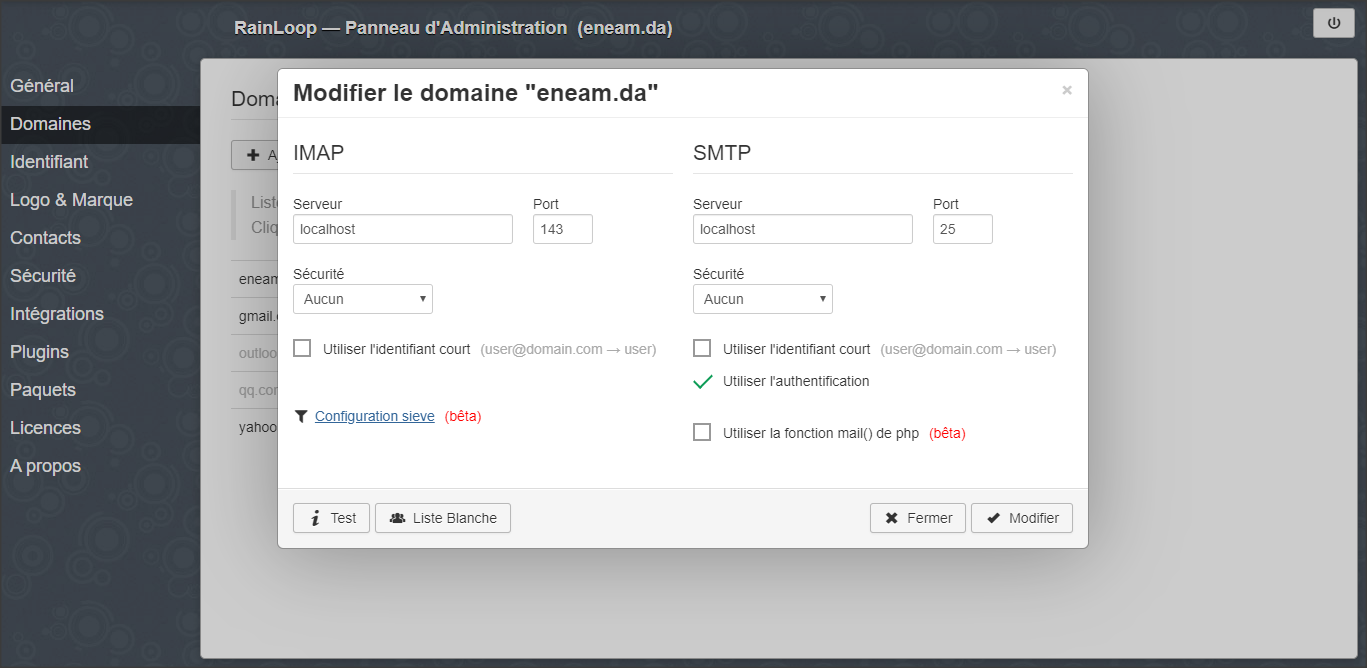
\includegraphics[width=483pt]{figure/configuration-domaine-rainloop.png}
	\caption{Ajout des serveurs mails dans rainloop}
\end{figure}

\section{Le site d'administration}
Le site d'administration va permettre de créer et de supprimer  les comptes emails, de voir la liste de quelques services (SMTP, IMAP, APACHE, NGINX ), leurr états,  de les arrêter ou de les éteindre. %Il a aussi la fonctionnalité qui va permettre à l'administrateur de voir les mails des étudiants qui est en cours de développement.
Il existe des solutions gratuites pour l'administration du mail comme \textbf{postfixadmin}
\subsection*{Les raisons pour lesquelles nous n'utilisons pas une solution existante}
%\subsection*{Pourquoi n'ai-je pas utilisé une solution existante ?}
\begin{itemize}
\item Les solutions existantes contiennent beaucoup de fonctionnalités que nous avons jugé inutile dans notre contexte. Par exemple nous n'avons pas besoin des alias. Nous ne voulons pas qu'un utilisateur soit en mesure d'accéder à son compte avec différents adresse mails.
%Prenons les alias. On conçoit difficilement qu'il puisse avoir d'alias de comptes (c'est-à-dire un alias d'un email ou un étudiant possédant plusieurs comptes).
\item L'apprentissage : nous allons comprendre les principes de base pour développer un site web d'administration de mails et écrire des scripts bash. Nous allons combiner toutes les technologies reçues lors de notre apprentissage pour produire un résultat.
%\item Le bonheur de coder: on va comprendre les principes de base pour coder un site d'administration de mails et écrire des scripts bash; ce qui est très intéressant et montre qu'on arrive à combiner toutes les technologies qu'on nous à enseigner lors des cours et dont on dispose pour produire un résultat ;
\item Postfixadmin est un outil puissant mais son interface est un peu vieillissant.
\item La flexibilité: étant donné que nous codons, nous allons adapter l'application à notre besoin.
\item Il existe des outils efficaces, complets mais pas gratuits et qui contiennent des fonctionnalités qui ne sont pas nécessaire pour nos besoins.\footnote{Beaucoup d'entreprises préfèrent souvent des solutions complètes, faciles d'utilisation comme cPanel. Mais ces outils sont à des prix très onéreux.}
\end{itemize}

\subsection*{Entités manipulés}
Nous utilisons le diagramme de classe du langage UML pour représenter les entités qui interagissent.
En effet, les utilisateurs virtuels représentent les utilisateurs de la messagerie et la classe Admin les adminitrateurs du système. Ces administrateurs sont des rôles et sont responsables de la gestion des utilisateurs.
\begin{figure}[H]
	\centering
	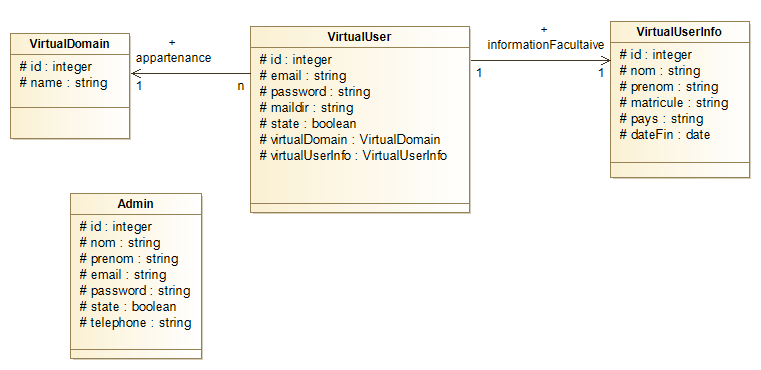
\includegraphics[scale=0.5]{figure/diagram-class.png}
	\caption{Diagramme de Classe UML du site d'administration}
\end{figure}
\subsection*{Configuration}
L'administrateur du système va exécuter des instructions depuis l'interface web et pour communiquer avec la machine \textbf{serveur} via l'interface web, il va appeler des scripts bash. Nous avons un script bash pour créer le répertoire d'un utilisateur, un autre pour supprimer un répertoire lors de la suppression d'un compte, un autre pour connaître l'état d'un service, un pour arrêter ou redémarrer un service. Voici le contenu du script qui redémarre un service :
\exempleConsoleFileBash{source/restartOrStopService.sh}

Pour permettre l'exécution de scripts bash depuis le web, il faut autoriser l'utilisateur web \emph{\textbf{www-data}} à lancer des scripts avec des droits administrateurs. Nous installons le programme sudo et nous ajoutons quelques lignes dans le fichier /etc/sudoers :
\begin{exempleConsole}
sudo apt-get install sudo 
#Les lignes dans /etc/sudoers
www-data ALL = NOPASSWD: /externe/www/html/www.admin.eneam.da/public_html/scripts/*
#On admet que tous nos scripts qui ont besoins des droits root sont dans ce répertoire	
\end{exempleConsole}

\section{Configuration du FTP  avec vsftpd}
\begin{exempleConsole}
sudo apt-get update
sudo apt-get install vsftpd
\end{exempleConsole}

Le fichier de configuration de vsftpd /etc/vsftpd.conf
\exempleConsoleFile{source/vsftpd.conf}

Nous créons le dossier /etc/vsftpd/ puis le fichier /etc/vsftpd/programmeur qui va contenir les directives pour connecter l'utilisateur virtuel \textbf{programmeur} au serveur FTP :
\exempleConsoleFile{source/programmeur}

\section{Spamassassin}
Spamassassin est un anti spam. Il va lire dans les logs et vérifier le nombre de tentatives de connexion échouée ou autres paramètres. Si on atteint ou dépasse un seuil, il bloque les connexions du client au serveur. Ce qui empêche les spammeurs d'utiliser le serveur pour envoyer du spam\footnote{Contenu, mail indésirable.}. Plus les règles établies sont strictes, plus les mails seront rejetés. 
\begin{exempleConsole}
apt-get install spamassassin
\end{exempleConsole}

Nous créons un utilisateur propre à spamassassin.
\begin{exempleConsole}
adduser spamd --disabled-login
\end{exempleConsole}

Le fichier /etc/default/spamassassin sera modifié.
\begin{exempleConsole}
ENABLED =1
OPTIONS="--create-prefs --max-children 5 --username spamd --helper-home-dir /home/spamd/ -s /home/spamd/spamd.log"
CRON =1
\end{exempleConsole}

Nous ajoutons les règles dans le fichier /etc/spamassassin/local.cf
\begin{exempleConsole}
rewrite_header Subject [***** SPAM _SCORE_ *****]
required_score 5.0
use_bayes 1
bayes_auto_learn 1
\end{exempleConsole}

\section{La base de données MariaDB}
Voici le script SQL complet qui gère notre domaine
\cesure
\exempleConsoleFileSQL{source/script-database-creation.sql}
\nocesure

\section{ Sécurité}
Nous allons écrire des règles iptables. La partie 2 du cours sécurisez votre réseau grâce aux VPN et firewall de Motta  \cite{ref17} traite du sujet. Nous créons le fichier /etc/init.d/regle-firewall :
%\exempleConsoleFile{"source/reglefirewall"}
\begin{exempleConsole}
#!/bin/sh
iptables-restore < /etc/iptables.test.rules
# On vide les règles déjà existantes
iptables -t filter -F
iptables -t filter -X

# On refuse toutes les connexions
iptables --policy FORWARD DROP
iptables --policy INPUT  DROP
iptables --policy OUTPUT  DROP
echo "On interdit tout"


# On autorise les connexions déjà établie
#iptables -A INPUT -m state --state RELATED,ESTABLISHED -j ACCEPT
#iptables -A OUTPUT -m state --state RELATED,ESTABLISHED -j ACCEPT

# On autorise le loop-back (localhost)
iptables -t filter -A INPUT -i lo -j ACCEPT
iptables -t filter -A OUTPUT -o lo -j ACCEPT
echo "On autorise le localhost"

#FTP
iptables -A INPUT -p tcp --dport 20 -j ACCEPT
iptables -A INPUT -p tcp --dport 21 -j ACCEPT
iptables -A OUTPUT -p tcp --sport 20 -j ACCEPT
iptables -A OUTPUT -p tcp --sport 21 -j ACCEPT
iptables -A INPUT -p tcp --dport 20000:20050 -j ACCEPT 
iptables -A OUTPUT -p tcp --sport 20000:20050 -j ACCEPT
echo "On autorise le FTP"

#SSH
iptables -A INPUT -p tcp --dport 22 -m conntrack --ctstate NEW,ESTABLISHED -j ACCEPT
iptables -A OUTPUT -p tcp --sport 22 -m conntrack --ctstate ESTABLISHED -j ACCEPT
echo "On autorise le SSH"

#SMTP et SMTPS, SMTP sur STARTLS
iptables -A INPUT -p tcp --dport 25 -m conntrack --ctstate NEW,ESTABLISHED -j ACCEPT
iptables -A INPUT -p tcp --dport 465 -m conntrack --ctstate NEW,ESTABLISHED -j ACCEPT
iptables -A INPUT -p tcp --dport 587 -m conntrack --ctstate NEW,ESTABLISHED -j ACCEPT
iptables -A OUTPUT -p tcp --sport 25 -m conntrack --ctstate ESTABLISHED -j ACCEPT
iptables -A OUTPUT -p tcp --sport 465 -m conntrack --ctstate ESTABLISHED -j ACCEPT
iptables -A OUTPUT -p tcp --sport 587 -m conntrack --ctstate ESTABLISHED -j ACCEPT
echo "On autorise le SMTP"

#HTTP et HTTPS
iptables -A INPUT -p tcp --dport 80 -m conntrack --ctstate NEW,ESTABLISHED -j ACCEPT
iptables -A INPUT -p tcp --dport 443 -m conntrack --ctstate NEW,ESTABLISHED -j ACCEPT
#iptables -A INPUT -p tcp --dport 7080 -m conntrack --ctstate NEW,ESTABLISHED -j ACCEPT
#iptables -A INPUT -p tcp --dport 7443 -m conntrack --ctstate NEW,ESTABLISHED -j ACCEPT
iptables -A OUTPUT -p tcp --sport 80 -m conntrack --ctstate ESTABLISHED -j ACCEPT
iptables -A OUTPUT -p tcp --sport 443 -m conntrack --ctstate ESTABLISHED -j ACCEPT
#iptables -A INPUT -p tcp --sport 7443 -m conntrack --ctstate NEW,ESTABLISHED -j ACCEPT
echo "On autorise le HTTP "

#IMAP
iptables -A INPUT -p tcp --dport 143 -m conntrack --ctstate NEW,ESTABLISHED -j ACCEPT
iptables -A INPUT -p tcp --dport 993 -m conntrack --ctstate NEW,ESTABLISHED -j ACCEPT
iptables -A OUUTPUT -p tcp --sport 143 -m conntrack --ctstate ESTABLISHED -j ACCEPT
iptables -A OUTPUT -p tcp --sport 993 -m conntrack --ctstate ESTABLISHED -j ACCEPT
echo "On autorise le IMAP"

## POP3
iptables -A INPUT -p tcp --dport 110 -m conntrack --ctstate NEW,ESTABLISHED -j ACCEPT
iptables -A INPUT -p tcp --dport 995 -m conntrack --ctstate NEW,ESTABLISHED -j ACCEPT
iptables -A OUTPUT -p tcp --sport 110 -m conntrack --ctstate ESTABLISHED -j ACCEPT
iptables -A OUTPUT -p tcp --sport 995 -m conntrack --ctstate ESTABLISHED -j ACCEPT
echo "On autorise le POP"

# NTP (pour avoir un serveur à l'heure)
iptables -t filter -A OUTPUT -p udp --dport 123 -j ACCEPT

# On autorise le ping
iptables -t filter -A INPUT -p icmp -j ACCEPT
iptables -t filter -A OUTPUT -p icmp -j ACCEPT
echo "On autorise le ping"

\end{exempleConsole}
\begin{comment}
\begin{exempleConsole}
iptables --policy FORWARD DROP
iptables --policy INPUT  DROP
iptables --policy OUTPUT  DROP
#FTP
iptables --append INPUT --protocol tcp --dport 21 -m conntrack --ctstate NEW,ESTABLISHED -j ACCEPT
#SSH
iptables --append INPUT --protocol tcp --dport 22 -m conntrack --ctstate NEW,ESTABLISHED -j ACCEPT
#SMTP et SMTPS SMTP sur STARTLS
iptables --append INPUT --protocol tcp --dport 25 -m conntrack --ctstate NEW,ESTABLISHED -j ACCEPT
iptables --append INPUT --protocol tcp --dport 465 -m conntrack --ctstate NEW,ESTABLISHED -j ACCEPT
iptables --append INPUT --protocol tcp --dport 587 -m conntrack --ctstate NEW,ESTABLISHED -j ACCEPT
#HTTP et HTTPS
iptables --append INPUT --protocol tcp --dport 80 -m conntrack --ctstate NEW,ESTABLISHED -j ACCEPT
iptables --append INPUT --protocol tcp --dport 443 -m conntrack --ctstate NEW,ESTABLISHED -j ACCEPT
iptables --append INPUT --protocol tcp --dport 7080 -m conntrack --ctstate NEW,ESTABLISHED -j ACCEPT
iptables --append INPUT --protocol tcp --dport 7443 -m conntrack --ctstate NEW,ESTABLISHED -j ACCEPT
#IMAP
iptables --append INPUT --protocol tcp --dport 143 -m conntrack --ctstate NEW,ESTABLISHED -j ACCEPT
iptables --append INPUT --protocol tcp --dport 993 -m conntrack --ctstate NEW,ESTABLISHED -j ACCEPT
#MYSQL
iptables --append INPUT --protocol tcp --dport 3306 -m conntrack --ctstate NEW,ESTABLISHED -j ACCEPT
\end{exempleConsole}
\end{comment}

Pour activer les règles iptables au démarrage du serveur nous créons le fichier /lib/systemd/system/firewall.service :
\begin{exempleConsole}
[Unit]
Description=Firewall
Requires=network-online.target
After=network-online.target
[Service]
User=root
Type=oneshot
RemainAfterExit=yes
ExecStart=/etc/init.d/regle-firewall.sh start
ExecStop=/etc/init.d/regle-firewall.sh stop
[Install]
WantedBy=multi-user.target	
\end{exempleConsole}

\section{Cas concret}\label{ref:casConret}
Nous allons illustrer l'utilisation du système par un exemple pratique. Voici l'énoncé.

\subsection{Enoncé}
%L'administrateur maître (master@eneam.da) va créer le compte administrateur admin@eneam.da.
Baké et Toto sont deux nouveaux étudiants de l'ENEAM. L'administrateur maître (master@eneam.da) va créer le compte administrateur \textbf{admin} (le login est admin@eneam.da et le mot de passe est \textbf{\_Admin229@}). L'administrateur \textbf{admin} va créer les comptes emails de Baké et Toto. Pour cela, il se connecte à la plateforme www.admin.eneam.da. Une fois les comptes créés, Baké va se connecter par le webmail et va ensuite envoyer un message à Toto. Toto va lui aussi se connecter et répondre au mail reçu. L'administrateur \textbf{admin} va supprimer le compte de Béréké. De même, il va consulter la liste des services et arrêter temporairement le service mail pour raison de maintenance.

\subsection{Pratique}
\begin{itemize}
\item L'administrateur maître se connecte au site d'administration \textbf{admin.eneam.da} et renseigne son mot de passe.
\begin{figure}[H]
	\centering
	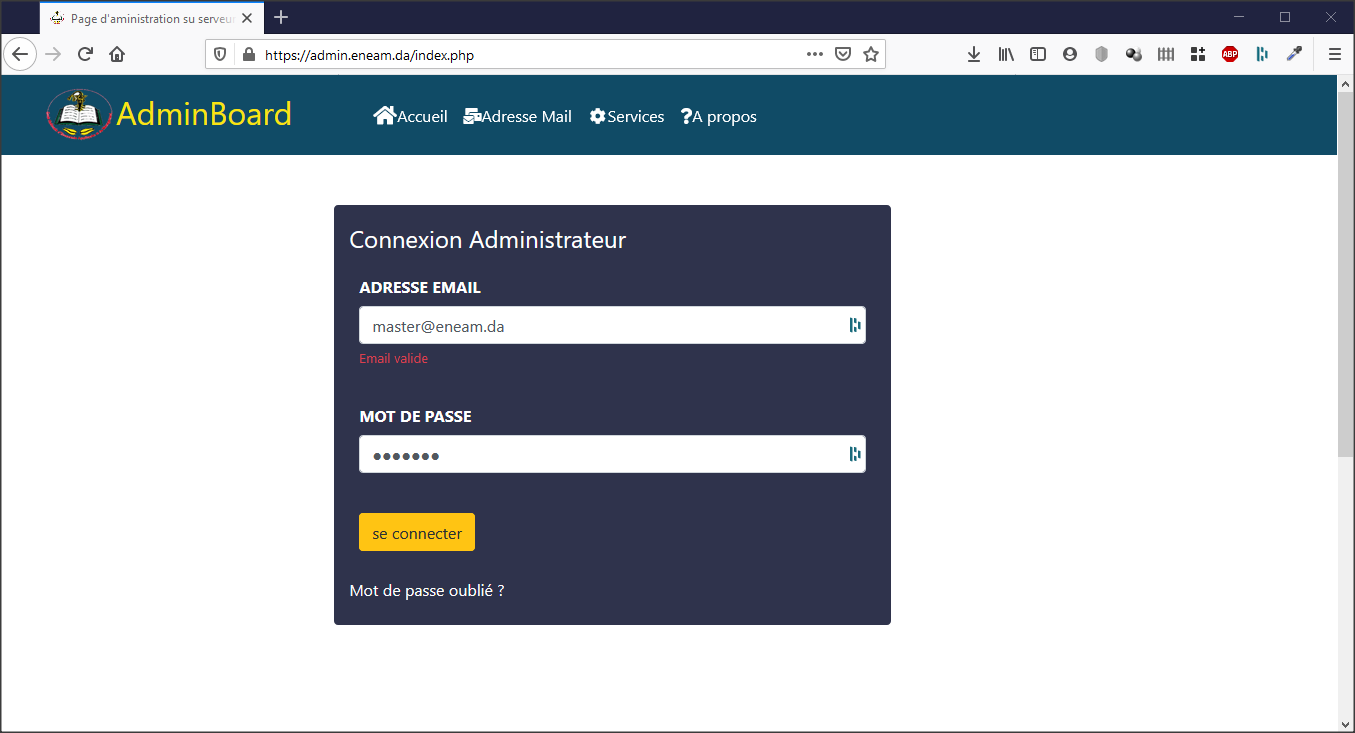
\includegraphics[width=483pt]{figure/connexion_master_admin.png}
	\caption{Connexion de l'administrateur master au site d'administration}
\end{figure}
\item Une fois connecté, il clique sur l'icône représentant l'utilisateur qui est située à l'extrême droite de l'écran et il choisit  le l'option "Gérer les administrateurs". 
\begin{figure}[H]
	\centering
	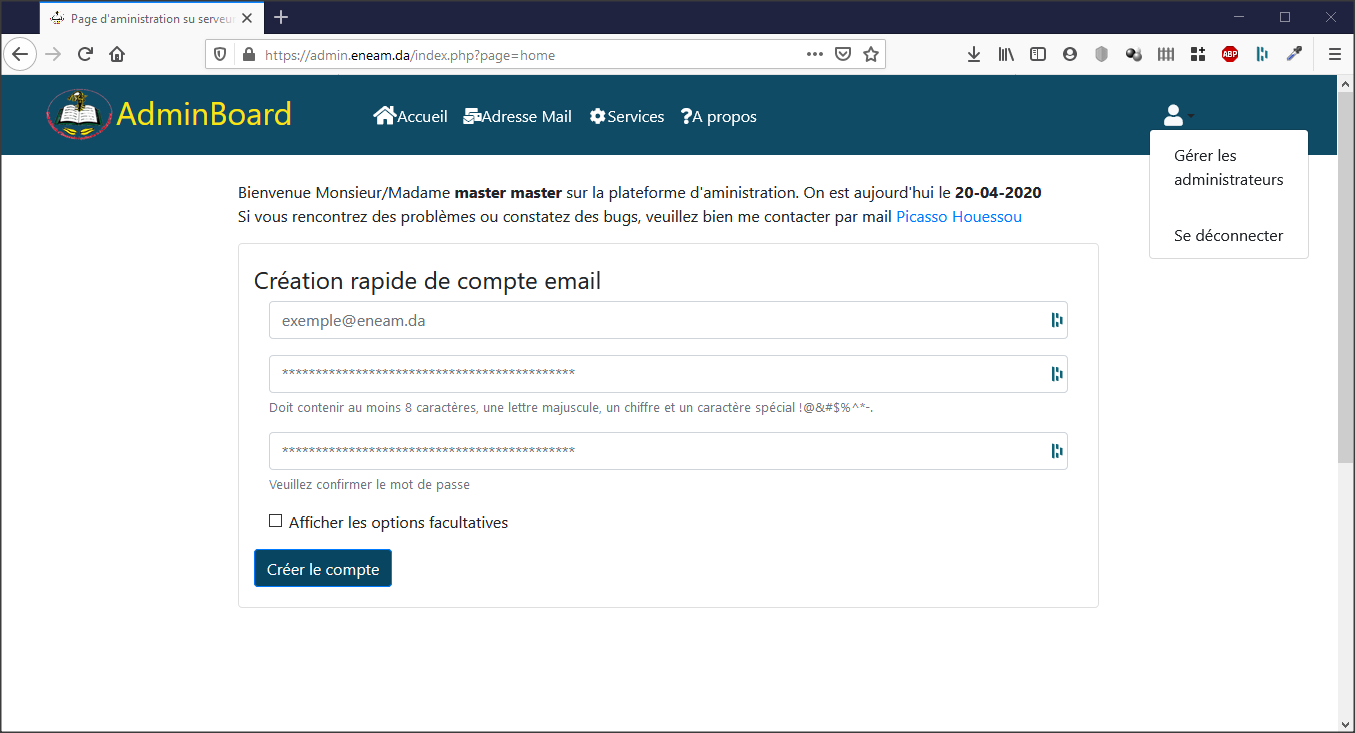
\includegraphics[width=483pt]{figure/gestion_administrateur_compte.png}
	\caption{Clic sur l'option Gérer les administrateurs}
\end{figure}
\item Il remplit le formulaire d'ajout d'un compte administrateur pour créer l'administrateur admin@eneam.da.
\begin{figure}[H]
	\centering
	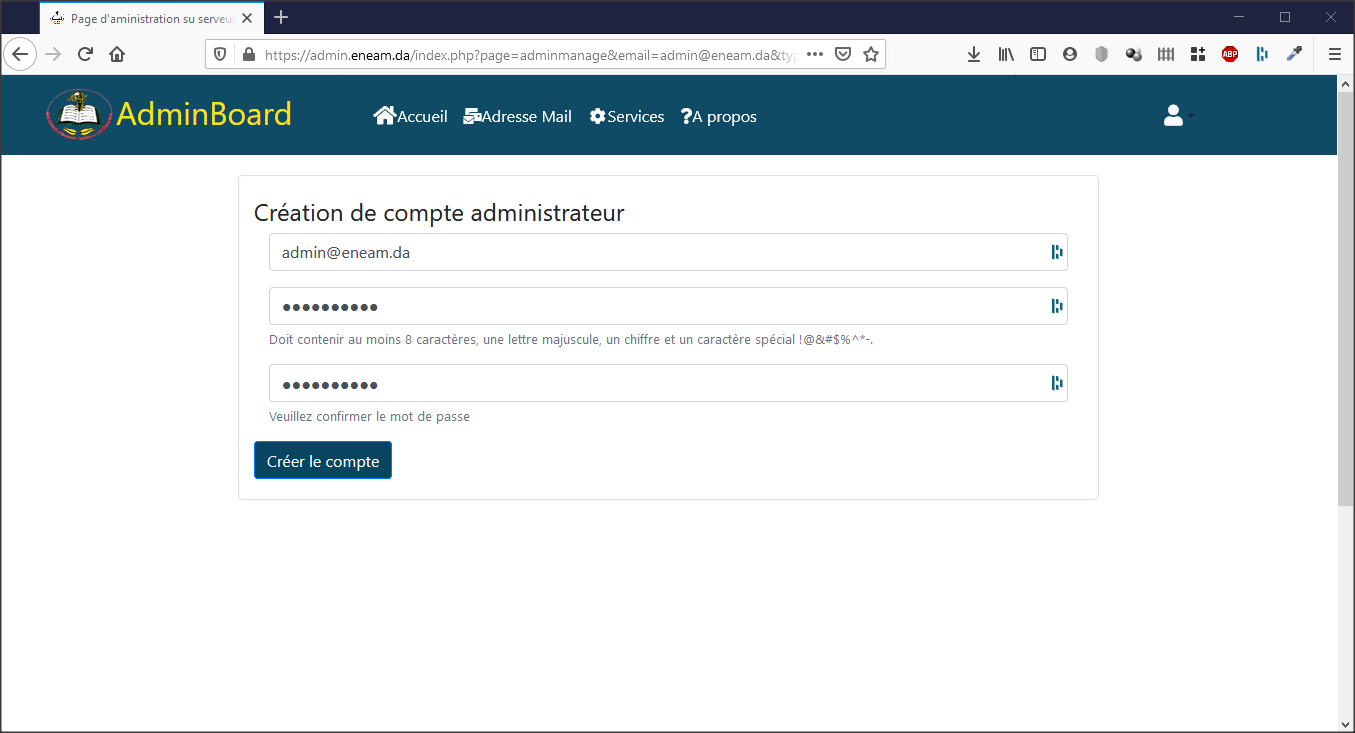
\includegraphics[width=483pt]{figure/master_creation_admin_compte.png}
	\caption{Création du compte administrateur admin}
\end{figure}
\item Il clique sur le bouton Créer le compte, ensuite le système renvoie un message pour notifier que le compte admin a été créé avec succès.
\begin{figure}[H]
	\centering
	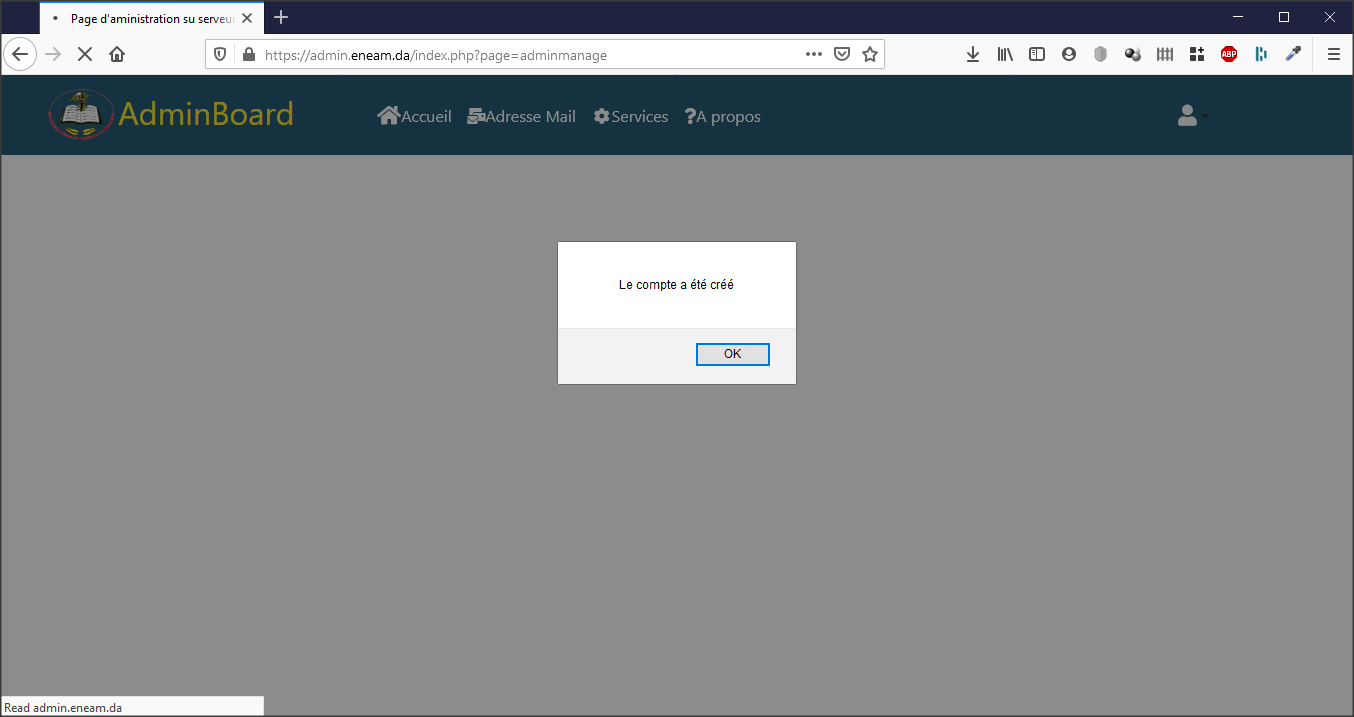
\includegraphics[width=483pt]{figure/master_creation_admin_compte_return_success.png}
	\caption{Message renvoyé lors de la création du compte administrateur admin}
\end{figure}
\item Création du compte mail de Baké: Nous allumons le poste admin. Nous ouvrons le navigateur et nous entrons l'adresse www.admin.eneam.da ou admin.eneam.da.
\item L'administrateur \textbf{admin} renseigne ses informations de connexion : son mot de passe est \textbf{\_Admin229@} et son adresse mail est \textbf{admin@eneam.da}.
\begin{figure}[H]
\centering
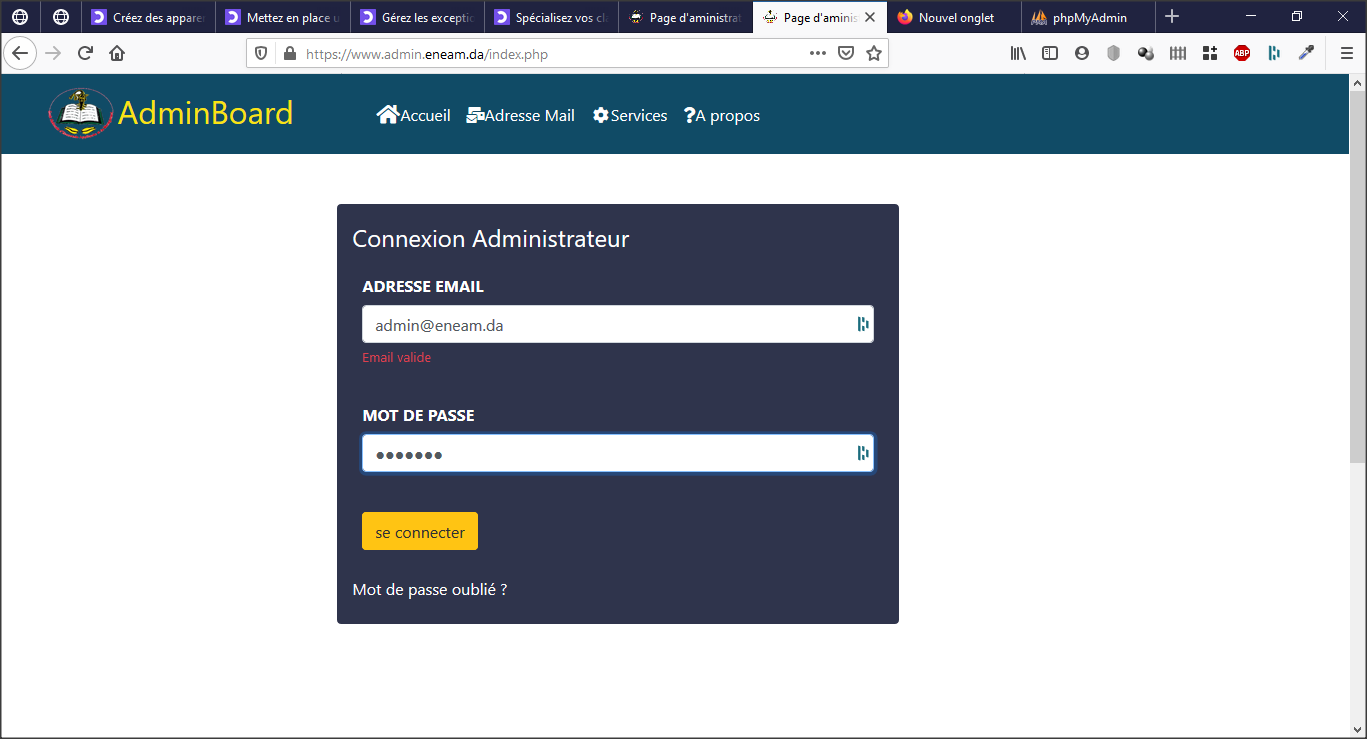
\includegraphics[scale=0.5]{figure/connexion_admin.png}
\caption{Connexion de l'administrateur au site d'administration}
\end{figure}
\item Sur la page d'accueil, il renseigne le compte mail qu'il veut créer. Ici nous allons mettre bake@eneam.da. Puis nous renseignons le mot de passe qui doit avoir une forte entropie\footnote{Il est obligatoire d'avoir au moins 8 caractères, un caractère spécial, une minuscule et une majuscule.}. On suppose ici \emph{Ba21@kesccT}. Nous confirmons le mot de passe.
\item Facultatif: Nous cochons la case Afficher les informations facultatives. Ce qui permet de renseigner le nom et prénom de l'étudiant, son numéro matricule, numéro de téléphone, la date d'expiration du compte.\footnote{Les comptes étant essentiellement pour des étudiants, il est  considéré qu'un compte est valide durant la période d'étude. On utilisera le programme \textbf{cron} pour désactiver automatiquement les comptes expirés.}
\begin{figure}[H]
\centering
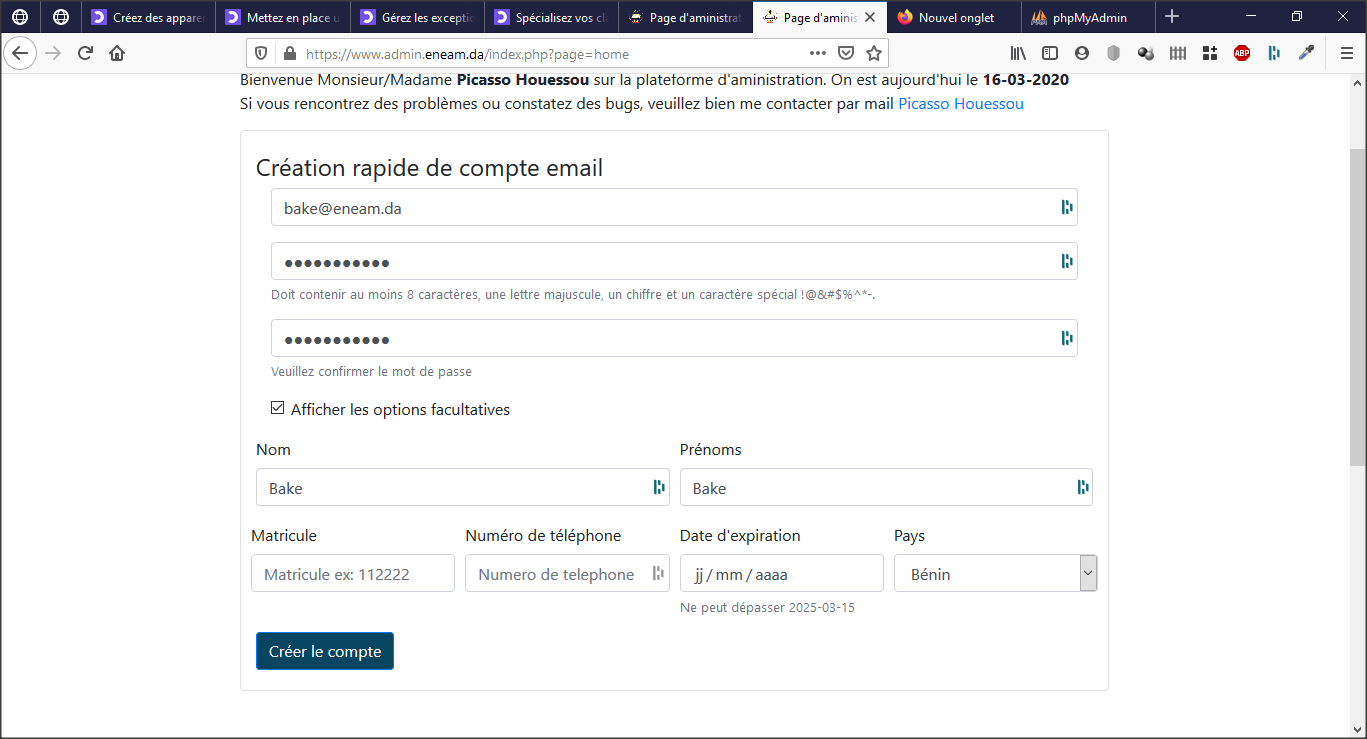
\includegraphics[width=483pt]{figure/creation_compte_bake.png} \\[1cm]
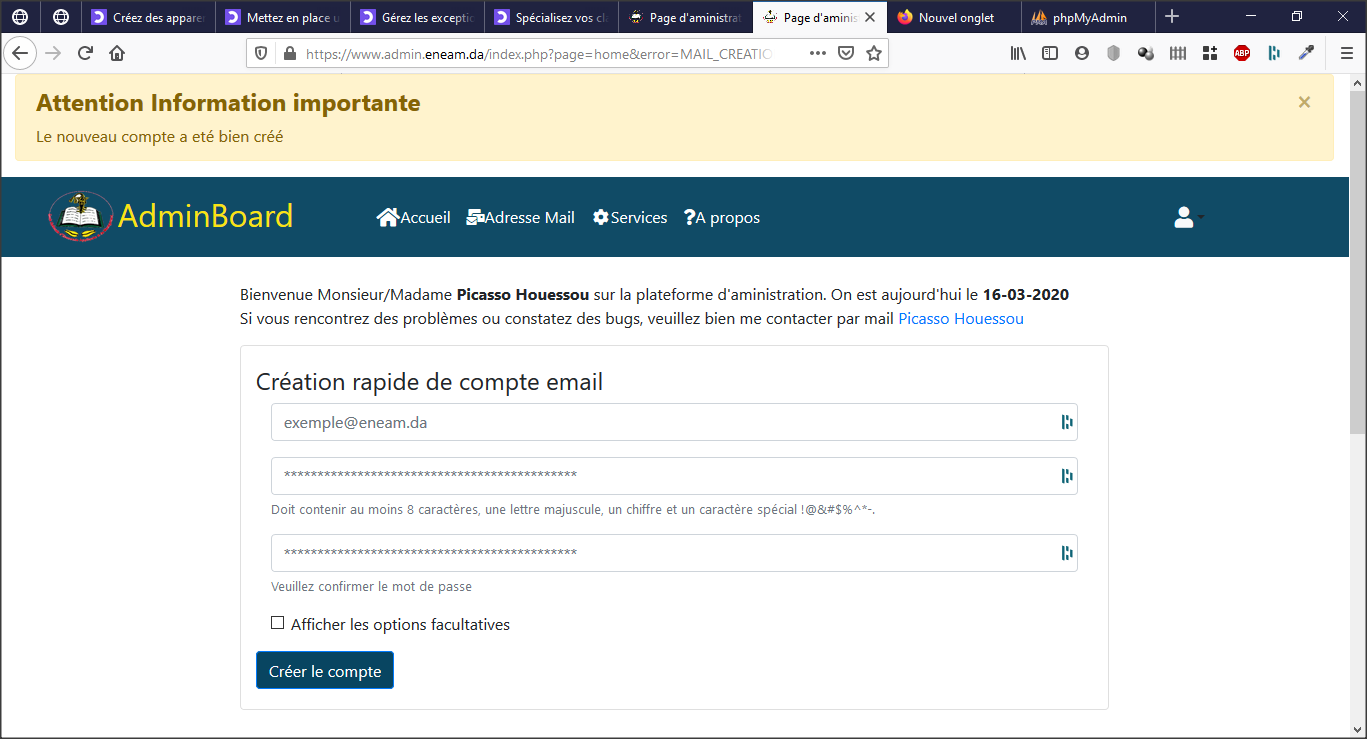
\includegraphics[width=483pt]{figure/retour_compte_cree.png}
\caption{Création du compte bake@eneam.da}
\end{figure} 
\item Nous cliquons sur le bouton \emph{Créer le compte}.
\item Le système renvoie une information pour notifier que le compte à été créé ou s'il a eu une erreur (par exemple si le compte existe déjà).
\item Il reprend la même opération pour Toto avec pour adresse mail toto@eneam.da et mot de passe to21@kesccT .
\item Baké tape www.eneam.da pour accéder au client webmail. Il saisit ses informations de connexion et se connecte.
\begin{figure}[H]
\centering
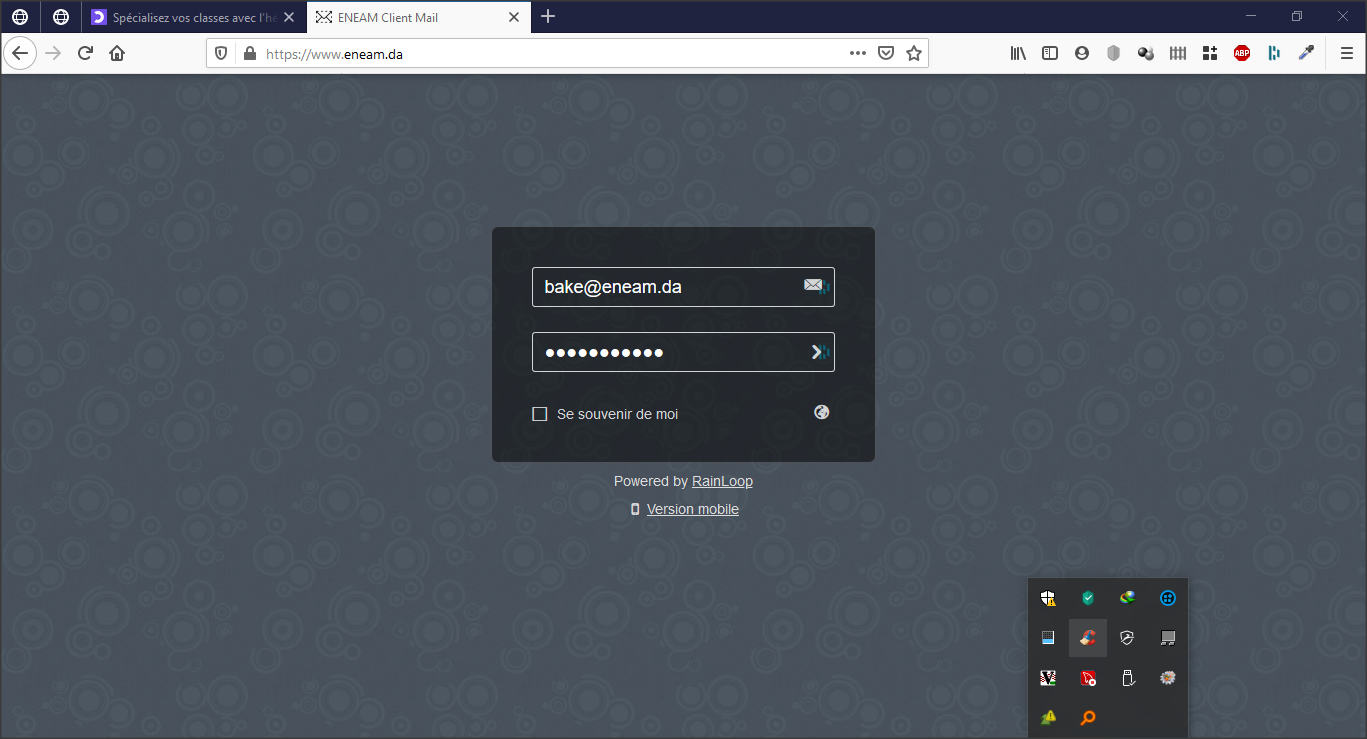
\includegraphics[width=483pt]{figure/connexion_bake_large_screen.png}
\caption{Connexion de Baké au client webmail}
\end{figure} 
\item Il crée un nouveau message à destination de Toto et l'envoie.
\begin{figure}[H]
\centering
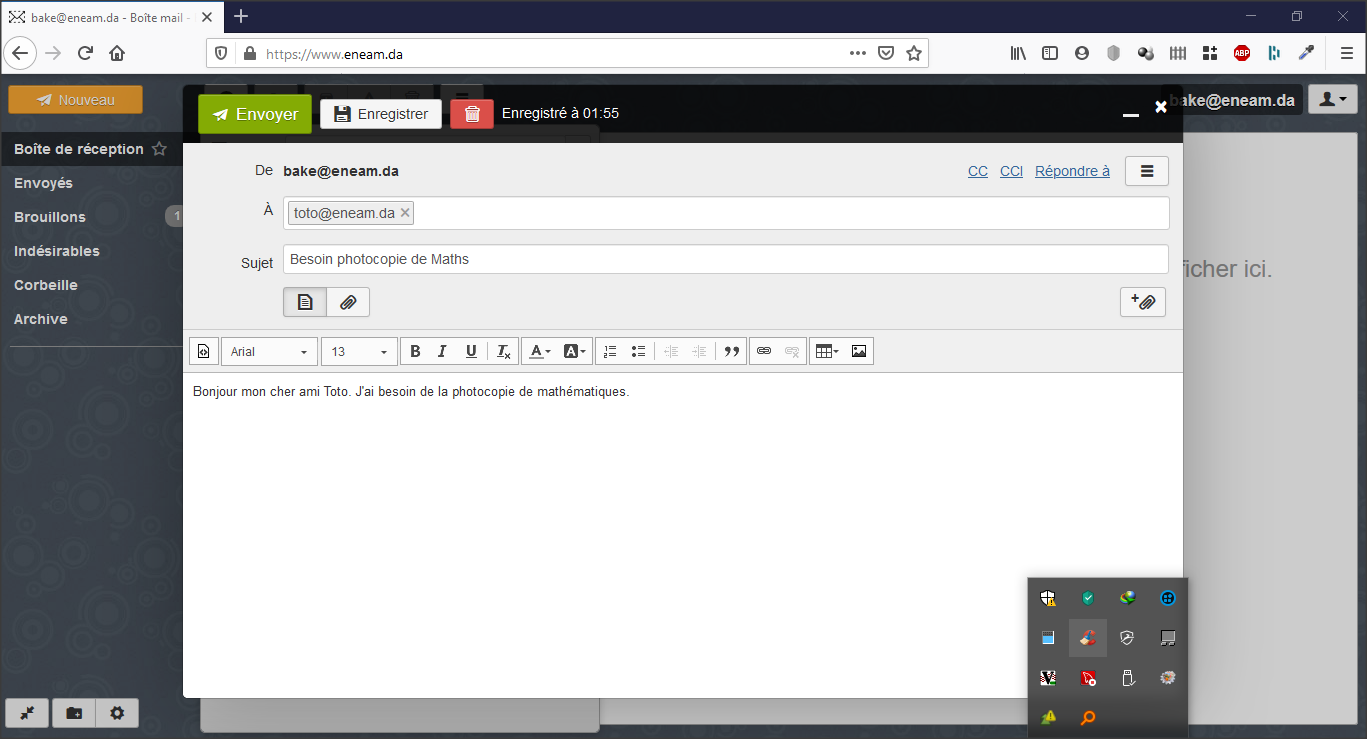
\includegraphics[width=483pt]{figure/bake_send_mail_to_toto1.png}
\caption{Envoi d'un mail de Baké à Toto}
\end{figure}

\item Toto se connecte et voit le message dans sa boite de réception.
\begin{figure}[H]
\centering
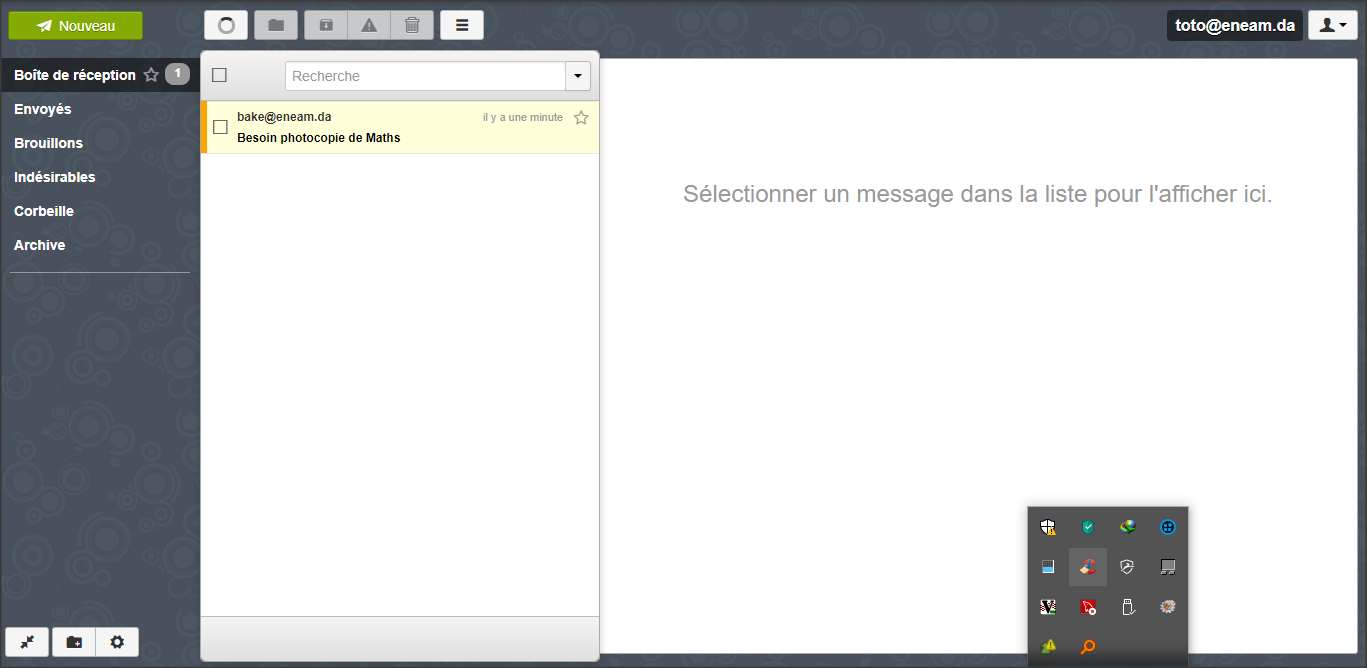
\includegraphics[width=483pt]{figure/toto_see_mail_from_bake1.png} \\[1cm]
\caption{Consultation de la boite de réception de Toto}
\end{figure} 
\item Toto répond au mail provenant de Baké.
\begin{figure}[H]
	\centering
	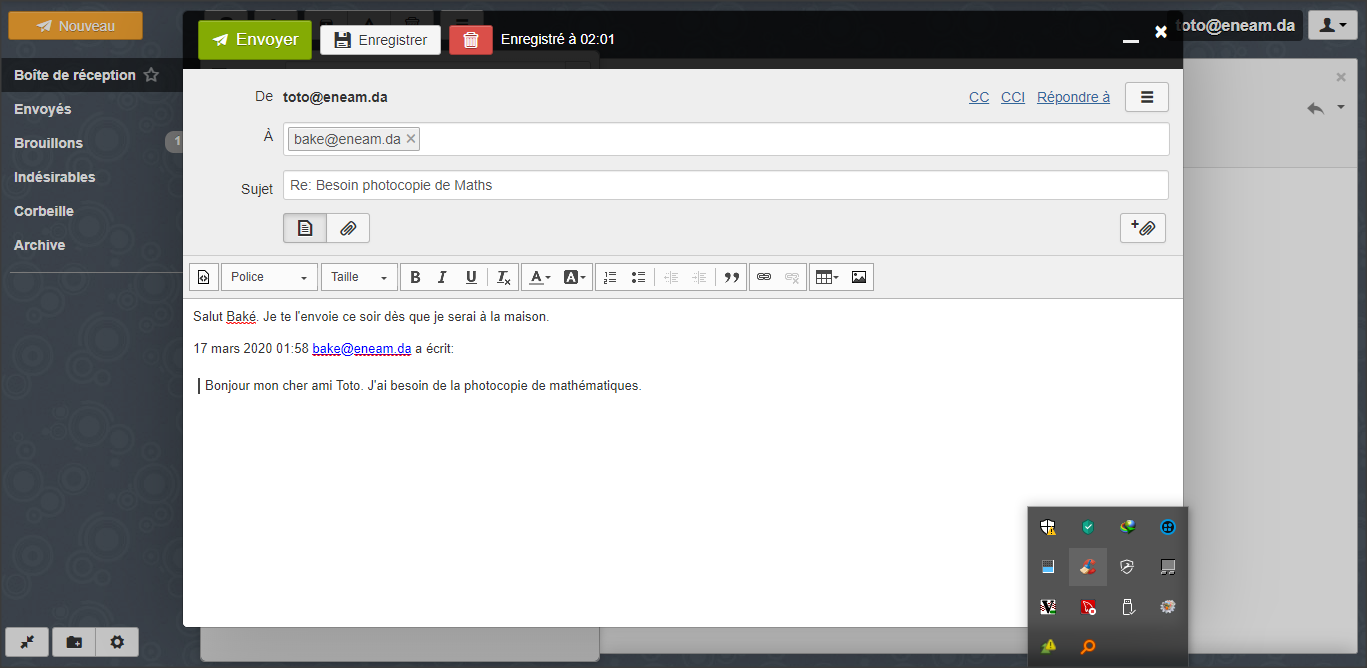
\includegraphics[width=483pt]{figure/toto_reply_to_bake1.png}
	\caption{Réponse de Toto au mail de Baké}
\end{figure} 

\begin{comment}
\item Toto se connecte voit le message de Baké et répond.
\begin{figure}[H]
\centering
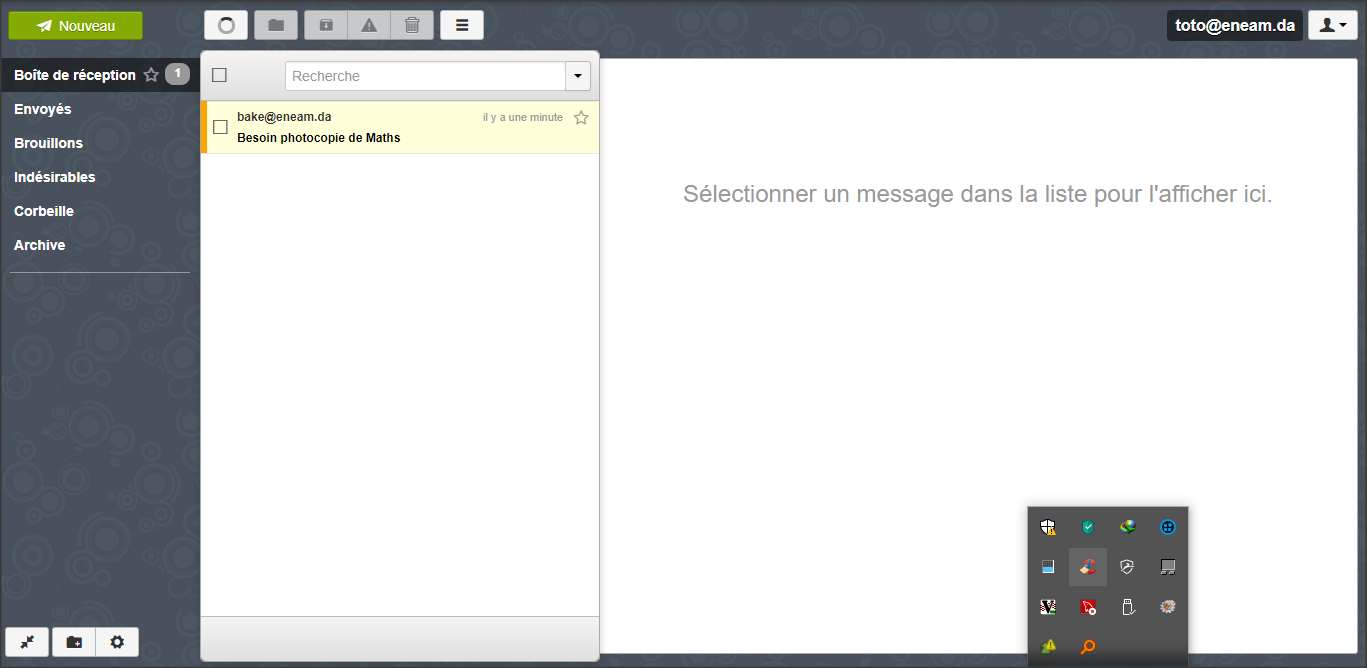
\includegraphics[width=483pt]{figure/toto_see_mail_from_bake1.png} \\[1cm]
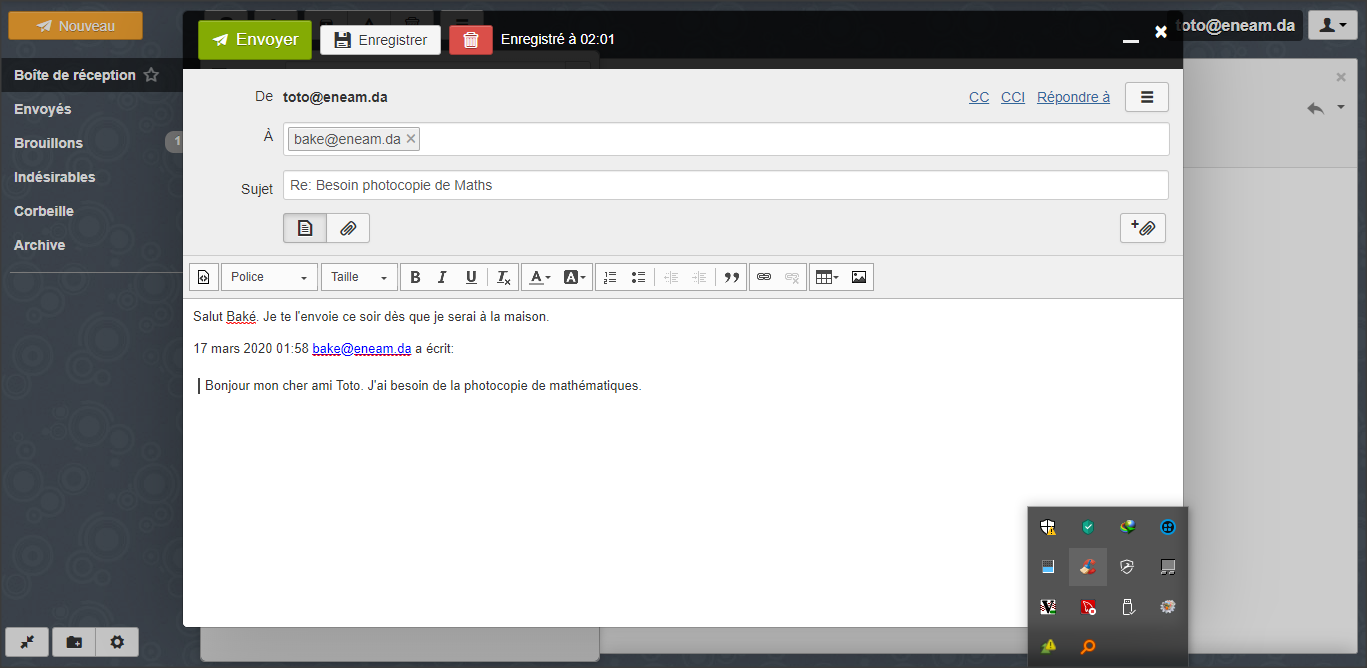
\includegraphics[width=483pt]{figure/toto_reply_to_bake1.png}
\caption{Lecture du mail reçu de Baké par Toto}
\end{figure} 
\end{comment}

\item L'administrateur \textbf{admin}  supprime le compte de Béréké : Pour cela il clique sur le menu Adresse mail. Ensuite, il recherche le compte de Toto et clique sur le bouton représenté par un bonhomme avec une croix. Une boîte de dialogue apparaît et demande de confirmer la suppression. Il clique sur oui supprimer. Des pop-ups apparaissent pour notifier si le compte a été supprimé. Il a la possibilité de les effacer ou de les enregistrer dans un fichier au format texte. % au cas où il voudrait écrire des notes plus tard. 
\begin{figure}[H]
\centering
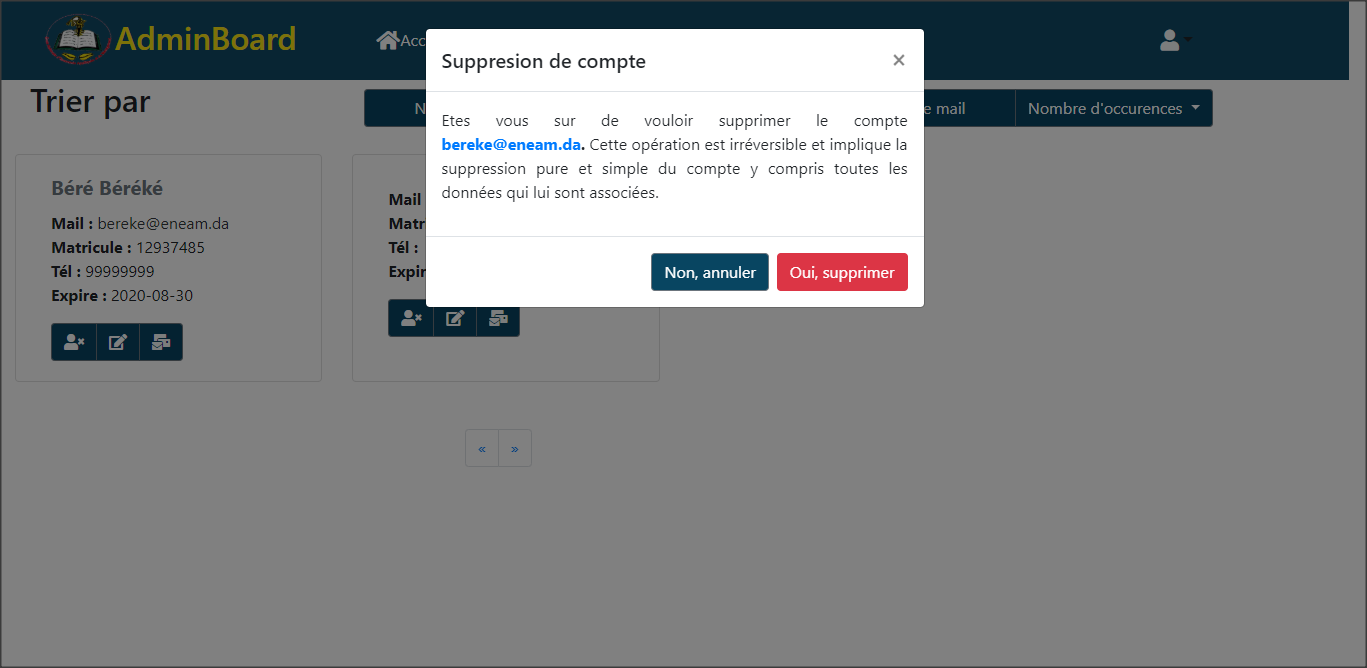
\includegraphics[width=483pt]{figure/admin_delete_bereke_acount1.png}
\caption{Suppression du compte de Béréké : confirmation de la suppression}
\end{figure} 
\begin{figure}[H]
	\centering
	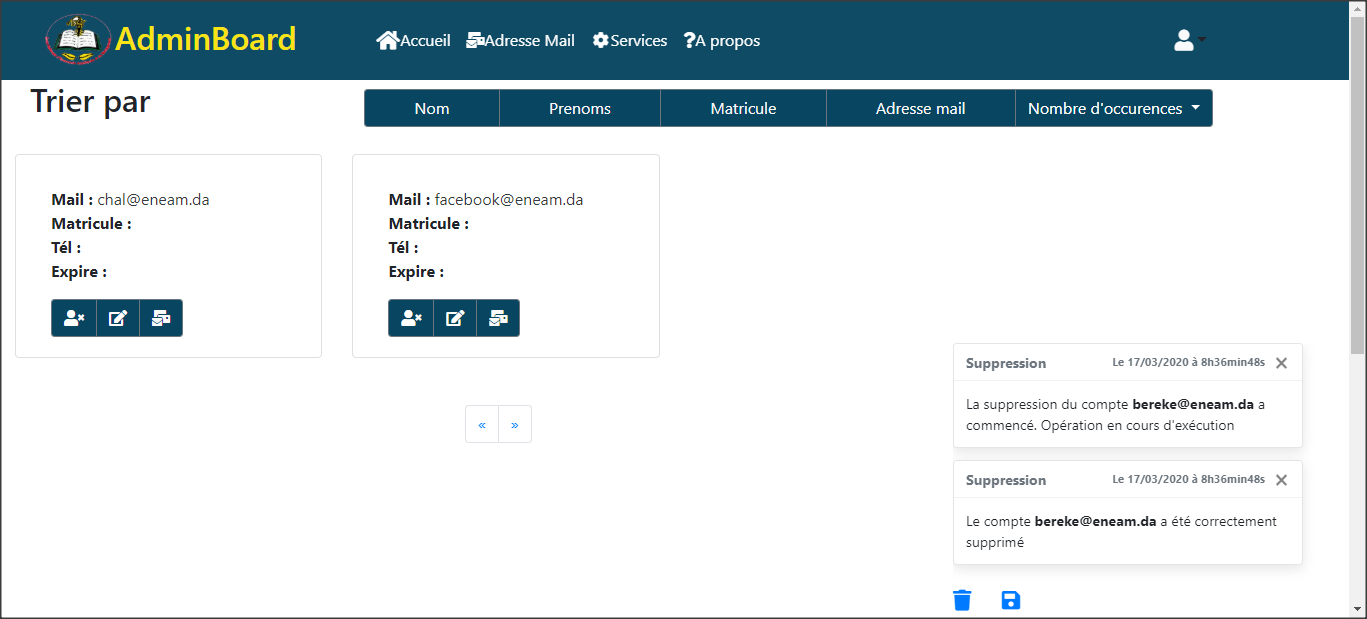
\includegraphics[width=483pt]{figure/admin_delete_bereke_acount2.png}
	\caption{Suppression du compte de Béréké: réponse du système}
\end{figure}  

\item L'administrateur \textbf{admin}  clique sur le menu Services. Il observe sur cette page 5 services. Le service Apache, Nginx, PHP7.2-FPM, Postfix, Dovecot. Il peut choisir de redémarrer un service en cliquant sur l'icône redémarrer dans le champ correspondant ou redémarrer tous les services à la fois en cliquant sur le bouton redémarrer tous les services. Il peut de même arrêter un service au besoin. Il est impossible d'arrêter les services web (Apache, Nginx, PHP7.2-FPM). En effet, il contrôle le serveur par l'interface web. S'il arrête donc les services web, il serait impossible de manipuler le serveur depuis le navigateur et il sera bloqué. C'est d'ailleurs la raison pour laquelle l'icône arrêter est désactivé pour ces trois services.
\begin{figure}[H]
\centering
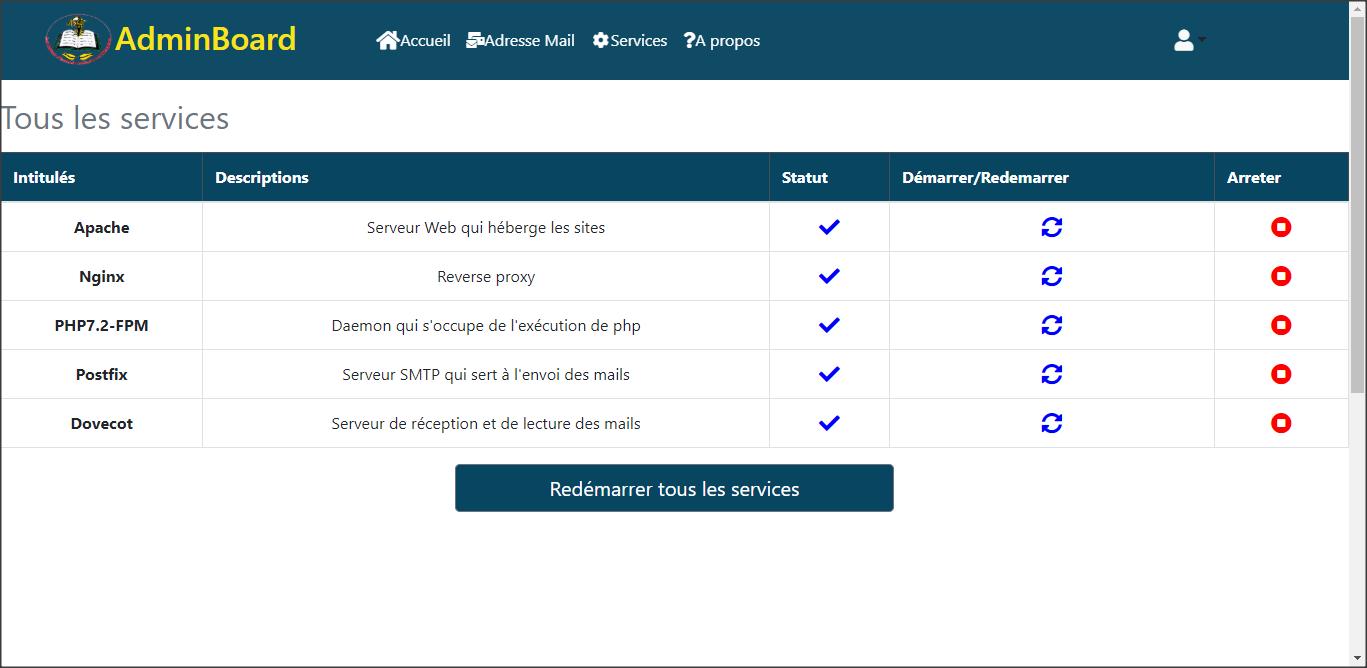
\includegraphics[width=483pt]{figure/admin_verify_state_of_service.png}
\caption{Vérification de l'état des services}
\end{figure}  

\item L'administrateur \textbf{admin}  arrête les services mails (Postfix et Dovecot)
\begin{figure}[H]
\centering
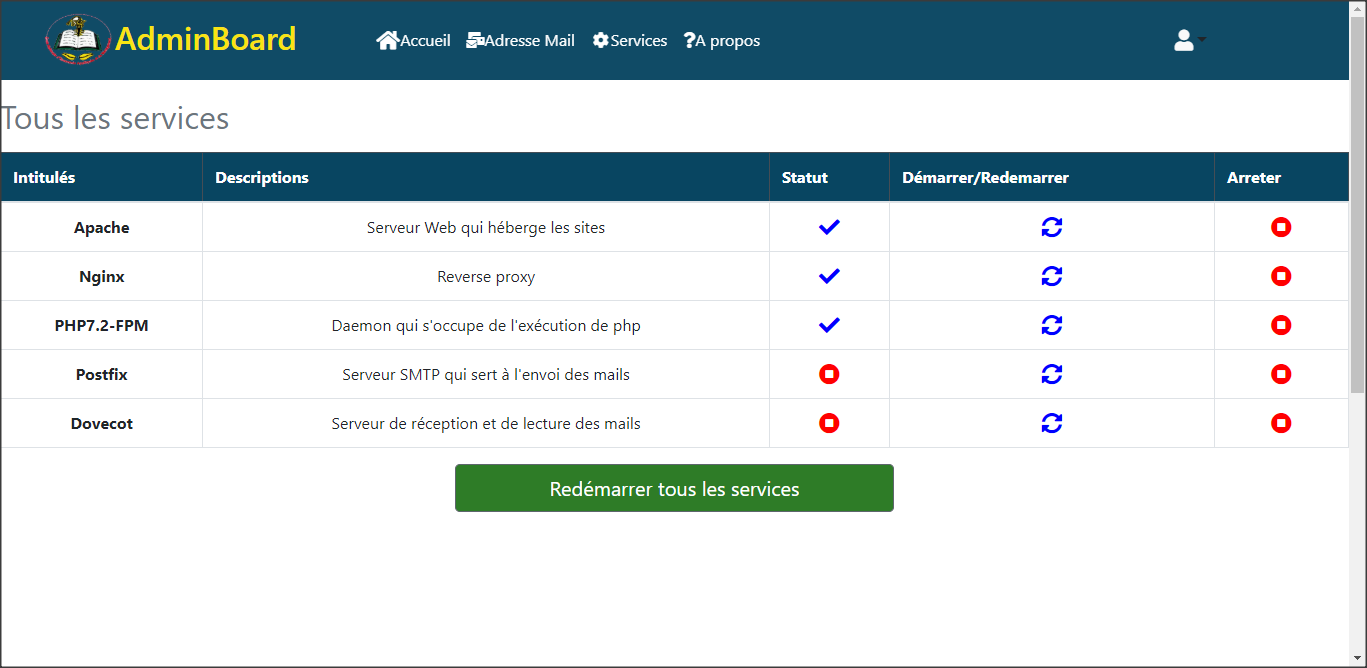
\includegraphics[width=483pt]{figure/admin_stop_service_mail.png}
\caption{Arrêt des services Postfix et Dovecot}
\end{figure}  

\item Il se déconnecte en cliquant sur l'icône située à l'extrême droite de l'écran et en appuyant sur se déconnecter. Pour des raisons de sécurité, il est aussi déconnecté automatiquement après une durée d'inactivité de 15 minutes. 
\end{itemize}

\begin{comment}
%\inputminted{frame = single, style = vim, autogobble,breaklines, bgcolor=bg, label=Console}{console}{vsftpd}
\chapter*{Conclusion}
Mon stage académique effectué au sein de JScom s'est révélé être une expérience marquante et m'a montré un aperçu des réalités quotidiennes en milieu professionnel.
J'ai mis en place un système d'envoi de mails pour faciliter les échanges au sein de l'ENEAM. Ce qui m'a permis d'explorer le vaste monde de l'administration système sous Linux. J'ai donc pu manipuler et découvrir plusieurs services réseaux. 
\end{comment}
\chapter*{Conclusion}
Nous avons déployé un serveur Linux Ubuntu qui permet l'envoi de messages électroniques. Le service de messagerie va contribuer à favoriser les échanges entre étudiants à l'école. En effet, par ce canal l'administration et les professeurs peuvent diffuser certaines informations aux étudiants sans risque d'altération ou de modification de l'information par les étudiants. La mise en place a nécessité d'installer un serveur de fichier, de configurer les services DHCP, DNS, Apache, MySQL, de faire de la virtualisation avec VMware et de la modélisation réseau grâce à GNS3, de configurer les protocoles SMTP et IMAP, de définir une politique de sécurité, d'utiliser la cryptographie pour sécuriser la communication et de développer un site web d'administration.

Notre stage académique effectué au sein de JScom s'est révélé être une expérience marquante et nous a montré un aperçu des réalités quotidiennes en milieu professionnel. Nous avons pu découvrir quelques outils d'administration système sous Linux. 
\addcontentsline{toc}{chapter}{Conclusion} %Ajout de Introduction dans la table des matieres

%Bibliographie
\nocite{ref1}
\nocite{ref2}
\nocite{ref3}
\nocite{ref4}
\nocite{ref5}
\nocite{ref6}
\nocite{ref7}
\nocite{ref8}
\nocite{ref9}
\nocite{ref10}
\nocite{ref11}
\nocite{ref12}
\nocite{ref13}
\nocite{ref14}
\nocite{ref15}
\nocite{ref16}
\nocite{ref17}
\bibliographystyle{plain}
\bibliography{bibliographie} % mon fichier de base de données s'appelle bibliogrphie.bib
\addcontentsline{toc}{chapter}{Bibliographie} %Ajout de Bibliographie dans la table des matieres
%Annexe
\end{document}
